\documentclass[10pt]{article}

\usepackage[margin=1in]{geometry}
\usepackage{booktabs}
\usepackage{tabularx}
\usepackage{multirow}
\usepackage{array}
\usepackage{tikz}
\usepackage{pgfplots}
\pgfplotsset{compat=1.18}
\usetikzlibrary{arrows.meta,positioning,fit,backgrounds,calc,matrix,decorations.pathreplacing}
\usepackage{amsmath}
\usepackage{amsthm}
\usepackage{xcolor}
\usepackage{listings}
\usepackage{caption}
\usepackage{subcaption}
\usepackage{hyperref}

\definecolor{codebg}{RGB}{246,246,246}
\definecolor{lockedcol}{RGB}{223,235,255}
\definecolor{writtencol}{RGB}{255,224,178}
\definecolor{ancestorcol}{RGB}{212,239,223}
\definecolor{barA}{RGB}{68,114,196}
\definecolor{barB}{RGB}{237,125,49}
\definecolor{barGood}{RGB}{84,130,53}
\definecolor{barBad}{RGB}{192,80,77}
\definecolor{curveA}{RGB}{68,114,196}
\definecolor{curveB}{RGB}{237,125,49}
\definecolor{curveC}{RGB}{84,130,53}
\definecolor{priorcol}{RGB}{223,235,255}
\definecolor{thispapercol}{RGB}{255,224,178}
\definecolor{partialcol}{RGB}{212,239,223}
\definecolor{opencol}{RGB}{240,240,240}
\definecolor{negcol}{RGB}{250,224,224}

\lstdefinestyle{verus}{
  backgroundcolor=\color{codebg},
  basicstyle=\ttfamily\scriptsize,
  breaklines=true,
  frame=single,
  rulecolor=\color{gray!40},
  showstringspaces=false,
  keywordstyle=\color{blue!70!black}\bfseries,
  commentstyle=\color{gray!70!black}\itshape,
  morekeywords={forall,requires,ensures,invariant,spec,proof,open,pub,fn,by,implies,decreases,ghost,tracked,let,mut,self,old,exec},
}
\lstset{style=verus}

\newtheorem{observation}{Observation}
\newtheorem{claim}{Claim}
\newtheorem{corollary}{Corollary}

\newcommand{\corten}[1]{\textsc{CortenMM\_#1}}
\newcommand{\vfn}[1]{\texttt{#1}}

\title{\bf Gated by Locking Structure, Not Fixed:
The Proof Cost of a Transactional Interface Across Three
Verified Concurrency Protocols in CortenMM}

\author{}
\date{}

\begin{document}
\sloppy
\maketitle

\begin{abstract}
CortenMM (SOSP~'25) is a machine-checked, high-performance concurrent
page table in Verus that reports both strong performance and a
tractable core proof by combining a single-layer abstraction,
fine-grained reader--writer locking, and a \emph{transactional}
interface --- one cursor, acquired once, shared across a caller-chosen
sequence of operations. As published, CortenMM does not measure what
this last decision costs, or what it buys. We take the
\emph{non-transactional} calling discipline CortenMM's own paper
attributes to Linux --- each operation independently acquires,
executes under, and releases its own lock, with no handle shared
across a sequence --- and apply it to three of CortenMM's concurrency
configurations (fine-grained reader--writer locking, a coarse
whole-tree lock, and an independently implemented RCU protocol),
constructing a verified variant for each. We hold every other design
decision, including all lower-level proof infrastructure, byte-for-byte
fixed relative to each variant's transactional baseline
(\emph{verification-preserving ablation}), so that comparing each
non-transactional variant against its own baseline, coordinate by
coordinate, attributes any change Verus reports to the interface
change alone. This comparison reveals a consistent pattern, not a
fixed cost: under fine-grained reader--writer locking, removing the
transactional interface exposes a frame-preservation proof obligation
the transactional design leaves implicit, costing $\sim$150 new lines
of proof code at 9 independently enumerable sites and raising the
obligation count from 149 to 150; under coarse, whole-tree locking,
the identical removal costs zero additional proof code and verifies at
an obligation count numerically identical to its transactional
counterpart (142 in both cases); and under RCU, an independently
implemented protocol exhibits the identical gap, repaired by the
identical fix, with zero regression in its own baseline's obligation
count (160). We formalize this as a threshold effect --- the cost is
gated by whether the locking protocol's ancestor range is degenerate
or structural, not a property of the interface change itself --- and
develop an amortized-fixed-cost model that a runtime evaluation
corroborates: the same interface removal costs $0.72\times$ to
$13.6\times$ (\texttt{mmap}) and up to $40\times$ (\texttt{mprotect})
the transactional convention's cost as operation-range size grows, and
that advantage collapses toward parity once realistic per-object work
(e.g.\ page faults) dominates, exactly as the model predicts. We
report these findings, the models that explain them, and their
explicit scope and non-claims --- including that three of our six
variants remain blocked from a clean 0-error result by two
documented, independent Verus tooling limitations --- positioned within a four-axis
classification of the memory-management design space that separates
interface atomicity from abstraction layering and concurrency protocol
as its own, independently variable axis.
\end{abstract}

\noindent\textbf{Keywords:} formal verification, proof engineering,
Rust, Verus, memory management, page tables, concurrency protocols,
transactional interfaces, ablation study, proof cost.



\section{Introduction}
\label{sec:intro}

Machine-checked verification of production-shaped systems software has
moved, in the last decade, from isolated microkernels~\cite{sel4} to
concurrent, performance-competitive data structures verified inside
real kernels~\cite{cortenmm}. This progress raises a question that
individual verified-system papers are not, by construction, positioned
to answer: when such a system reports both strong performance and a
tractable proof, \emph{which of its design decisions is responsible for
which property}? A system that bundles several decisions together ---
a data-structure abstraction, a concurrency protocol, and an interface
discipline --- reports their \emph{combined} effect; it does not, on its
own, tell a reader building the next such system which decision to
keep if resources allow only one.

CortenMM~\cite{cortenmm} is a sharp instance of this question.
Its page table collapses the usual two-level abstraction (a VMA
structure layered over a hardware page table) into one single-layer
structure, uses fine-grained per-level reader--writer locking, and
exposes callers a \emph{transactional} cursor --- one handle, acquired
once, shared across a caller-chosen sequence of operations --- and
reports both high performance and a machine-checked core proof in
Verus~\cite{verus}. The paper argues informally that the single-layer abstraction is
what makes verification tractable. It does not measure whether the
locking protocol or the transactional interface independently
contribute to that tractability, whether either contributes
independently to performance, or --- despite implementing more than
one concurrency protocol itself (reader--writer locking and RCU) ---
whether any such contribution is a property of one protocol or of the
class of protocols it belongs to.

\paragraph{This paper's approach.} CortenMM's own paper identifies,
without measuring, the alternative to its transactional design: the
\emph{non-transactional} calling discipline it attributes to Linux, in
which each operation independently acquires, executes under, and
releases its own lock, sharing no handle across a sequence. We take
this existing, already-attributed-to alternative and apply it to three
of CortenMM's own concurrency configurations --- fine-grained
reader--writer locking, a coarse whole-tree lock, and RCU --- to
construct a verified non-transactional variant of each
(\S\ref{sec:method:variants}). The methodological work is in making
this comparison sound: each variant is built under
\emph{verification-preserving ablation}, changing exactly the interface
axis while every other line of code --- including all lower-level
proof infrastructure --- remains byte-for-byte identical to that
variant's own transactional baseline, verified with the identical
toolchain and configuration (\S\ref{sec:method:principle}). Comparing
each non-transactional variant against its own baseline, coordinate by
coordinate, is what lets us attribute any change Verus reports to the
interface change alone, and comparing the resulting pattern
\emph{across} the three protocols is what lets us ask whether that
attribution is a property of one protocol or of a class. We also boot
each variant as a kernel image to measure runtime behavior
(\S\ref{sec:method:bench}), and develop a formal cost model that
explains the pattern the six variants exhibit and states, precisely,
what it does and does not predict (\S\ref{sec:theory}).

\paragraph{Findings.} Table~\ref{tab:intro-summary} summarizes our four
research questions and their answers; \S\ref{sec:eval} reports the full
evidence for each.

\begin{table}[h]
\centering
\small
\begin{tabularx}{\textwidth}{@{}l >{\raggedright\arraybackslash}p{3.6cm} >{\raggedright\arraybackslash}X@{}}
\toprule
\textbf{RQ} & \textbf{Question} & \textbf{Finding} \\
\midrule
RQ1 (\S\ref{sec:eval:gap1}) &
  Abstraction vs.\ locking protocol &
  Separable: \corten{coarse} (whole-tree lock) verifies with 142
  obligations vs.\ \corten{rw}'s 149 ($-5\%$); the same swap degrades
  throughput to 35--50\% of \corten{rw}'s under contention. Verifiability
  tracks the abstraction; performance tracks the locking protocol. \\
\addlinespace
RQ2 (\S\ref{sec:eval:gap4}) &
  Transactional interface's proof cost &
  Removing it (\corten{nontxn}) requires $\sim$150 new lines of proof
  code across 9 independent write/exit sites
  (Table~\ref{tab:gap4-sites}) and raises the obligation count from
  149 to 150 --- but only under fine-grained locking. The missing
  fourth cell, \corten{coarse-nontxn}, requires \emph{zero} new proof
  code and verifies at exactly 142, identical to \corten{coarse}: the
  cost is a threshold effect of the locking protocol's structure
  (\S\ref{sec:theory:proof}), not a fixed cost of removing the
  interface. \\
\addlinespace
RQ3 (\S\ref{sec:eval:rcu}) &
  Generalization across protocols &
  \corten{rcu}'s independently written \vfn{wf\_push\_level} is missing
  the identical range clause \corten{rw}'s is, and is repaired by the
  identical fix, with zero regression (160 obligations, unchanged).
  \corten{nontxn}, \corten{coarse-nontxn}, and \corten{rcu-nontxn} are all
  blocked from 0 errors by two distinct, documented residual Verus
  tooling limitations (\S\ref{sec:eval:threats}), not by any logical gap. \\
\addlinespace
RQ4 (\S\ref{sec:eval:perf}) &
  Runtime impact &
  Real but conditional: non-transactional calling costs
  $0.72\times$--$13.6\times$ (\vfn{mmap}) and up to $3.4\times$--$40\times$
  (\vfn{mprotect}) the transactional cost as range size grows from 1 to
  64 pages, consistent with an amortized-fixed-cost model
  (\S\ref{sec:theory:runtime}) that also predicts, and an
  allocator-arena workload confirms, that the advantage collapses
  toward $1\times$ once realistic per-object cost (e.g.\ page faults)
  dominates. \\
\bottomrule
\end{tabularx}
\caption{This paper's four research questions and findings, each
detailed with full evidence in \S\ref{sec:eval}.}
\label{tab:intro-summary}
\end{table}

\paragraph{Why the interface axis is its own axis.} Prior classification
of memory-management designs separates an \emph{abstraction} axis
(how many layers sit between the caller and hardware) from a
\emph{concurrency-protocol} axis (what serializes concurrent access).
\S\ref{sec:related:mece} situates this paper's work on a third,
orthogonal axis --- \emph{interface atomicity}, whether operations share
one locked handle across a sequence or each reacquire independently ---
that we argue deserves separate treatment because its proof-cost effect
(RQ2/RQ3) is not explained by either of the other two: it is
\emph{gated} by the concurrency-protocol axis (Table~\ref{tab:matrix}),
but is not itself a property of that axis, and it is orthogonal to the
abstraction axis entirely (every variant in this paper fixes the
single-layer abstraction and varies only locking and interface). Among
the Verus-verified systems we are aware of in this space
(Figure~\ref{fig:mece-grid}), we found none that instantiates
\emph{both} sides of the interface-atomicity axis the way CortenMM
does: \vfn{verified-nrkernel}~\cite{nrkernel} is single-threaded, and
\vfn{node-replication}~\cite{nr}'s public interface is
per-operation by construction. We report this as a limit on how far
RQ2/RQ3's finding can currently be checked to generalize
(\S\ref{sec:eval:threats}), not as evidence against it.

\paragraph{Contributions.} This paper contributes:
\begin{itemize}
  \item Applying an existing, already-attributed-to design (the
    non-transactional locking discipline CortenMM's own paper
    associates with Linux) to three of CortenMM's concurrency
    configurations, and, by comparing each resulting variant against
    its own transactional baseline coordinate by coordinate, showing
    that the proof cost of this design change is \emph{not} a fixed
    property of the interface: it is a threshold effect, gated by
    whether the underlying locking protocol's ancestor range is
    degenerate (a coarse, whole-tree lock, where the cost is exactly
    zero, \S\ref{sec:eval:gap4}) or structural (fine-grained
    reader--writer locking or RCU, where the cost is real and, across
    the two independently implemented structural protocols we tested,
    consistent in shape and repair, \S\ref{sec:eval:rcu}). Constructing
    the degenerate-protocol comparison point required first building
    and verifying \corten{coarse} (\S\ref{sec:eval:gap1}), whose own
    finding --- that verifiability tracks the abstraction layer and not
    the locking protocol --- is a supporting result this threshold
    effect depends on, not an independent claim of equal weight.
  \item \emph{Verification-preserving ablation}
    (\S\ref{sec:method:principle}): the methodological discipline ---
    change exactly one design axis, verify every resulting variant
    with the identical toolchain and configuration, keep every other
    line of code, including all lower-level proof infrastructure,
    byte-for-byte identical to that variant's own baseline --- that
    makes the coordinate-by-coordinate comparison above valid rather
    than confounded. Under it, we construct and verify six variants of
    CortenMM. \corten{rw}, \corten{coarse}, and \corten{rcu} verify with
    0 errors; \corten{nontxn}, \corten{coarse-nontxn}, and
    \corten{rcu-nontxn} have their core frame-preservation property
    fully proved but are blocked from a clean 0-error result by two
    distinct, documented, reproducible tooling limitations
    (\S\ref{sec:eval:threats}) --- both present in \corten{coarse-nontxn}
    simultaneously, which is how we confirmed they are two issues and
    not one (\S\ref{sec:method:variants}, \S\ref{sec:eval}).
  \item An exact, mechanistic characterization of the proof obligation
    that a transactional interface lets remain implicit --- a
    frame-preservation property over the cursor's ancestor range --- and
    a uniform proof pattern (step-fact/transitivity,
    \S\ref{sec:method:sites}) for discharging it at every one of the 9
    sites identified for \corten{nontxn} (Table~\ref{tab:gap4-sites}),
    and, independently, at the structurally identical
    \vfn{wf\_push\_level} gap we located and repaired in \corten{rcu}
    (\S\ref{sec:eval:rcu}) using the same fix.
  \item A formal threshold-effect account (\S\ref{sec:theory:proof})
    and an amortized-fixed-cost runtime model
    (\S\ref{sec:theory:runtime}) that together explain, without fitting
    any parameter to the measured data, both the proof-cost and the
    runtime results in \S\ref{sec:eval}, and state explicitly what they
    do not claim to predict (\S\ref{sec:theory:scope}) --- including
    that we tested three of the four concurrency-protocol categories in
    our own classification (\S\ref{sec:related:mece}), not all four,
    and make no claim about the untested one (replication) or about
    intermediate points between degenerate and structural locking.
  \item Four independent, reproducible artifact-infrastructure findings
    surfaced in the course of this work (a cross-tree build-path
    pollution bug in the artifact's Nix/Cargo tooling, a guest-runtime
    startup fault affecting any non-\vfn{pthread}-linked static
    binary, an intermittent kernel-build failure root-caused to a
    registry-mirror-shadowing conflict between a workspace-local and a
    registry-published copy of the same crate --- with a permanent fix
    now applied automatically by this artifact's build scripts --- and
    a corrected --- initially
    misdiagnosed --- account of an \vfn{mprotect}-related failure later
    traced to the \vfn{pthread} issue above), reported for the
    artifact's maintainers independently of this paper's main claims.
\end{itemize}

\paragraph{Organization.} \S\ref{sec:method} presents the ablation
methodology and the six constructed variants in full, code-aligned
detail. \S\ref{sec:eval} reports proof-cost and runtime results for
each research question. \S\ref{sec:theory} develops the two models that
explain those results. \S\ref{sec:related} positions this paper's
contribution within the four-axis design space it studies. We close
with the threats to validity already summarized above
(\S\ref{sec:eval:threats}) and directions the threshold-effect and
amortized-cost models suggest for future ablations beyond the two
protocols and three workloads this paper covers.



\section{Methodology}
\label{sec:method}

This section describes \emph{verification-preserving ablation} as a
general technique (\S\ref{sec:method:principle}), the concrete
CortenMM cursor abstraction that our ablations act on
(\S\ref{sec:method:cursor}), how each of the six variants evaluated in
\S\ref{sec:eval} was constructed (\S\ref{sec:method:variants}), the
specific proof obligation that non-transactional ablation exposes and
the general repair technique we developed for it
(\S\ref{sec:method:repair}--\S\ref{sec:method:sites}), and our runtime
benchmark methodology (\S\ref{sec:method:bench}). Every code fragment
in this section is quoted, not paraphrased, from the artifact crates we
built; identifiers match the source exactly.

\subsection{Verification-Preserving Ablation: Design Principles}
\label{sec:method:principle}

Given a verified system $S$ with a design decision $D$ (e.g., ``operations
share one lock across a caller-chosen sequence'' or ``the tree is locked
level-by-level''), we want to measure $D$'s independent contribution to
$S$'s proof cost and runtime behavior. A naive ablation --- writing a new
system $S'$ without $D$ from scratch, or hand-modifying $S$ until it
compiles --- confounds the answer: differences in obligation count
between $S$ and $S'$ may be attributable to $D$, to incidental
rewriting, or to a different verifier configuration. Verification-preserving
ablation enforces three constraints designed to eliminate these
confounds:

\begin{enumerate}
  \item \textbf{Copy, don't rewrite.} $S'$ begins as a byte-for-byte
    copy of $S$. Every subsequent edit is applied as a minimal,
    localized diff against files that implement $D$ or are its direct
    callers; every file that does not mention $D$ --- including all
    lower-level proof infrastructure shared by every variant
    (\vfn{node\_helper}, \vfn{ghost\_tree}, page-table-node guard
    types) --- is left untouched. \S\ref{sec:method:variants} reports
    the exact file-level diff for each variant we built.
  \item \textbf{Same verifier, same flags.} $S'$ is checked with the
    identical pinned Verus/Rust toolchain, identical \texttt{rlimit},
    and identical \texttt{cargo xtask verify} invocation as $S$; no
    variant receives special-cased verifier configuration except where
    \S\ref{sec:eval:threats} explicitly reports one as a residual
    tooling workaround attempt.
  \item \textbf{Preserve executable semantics.} Where the ablation
    concerns an \emph{interface} rather than a locking mechanism (e.g.,
    \corten{nontxn} in \S\ref{sec:eval:gap4}), the underlying executable
    primitives (\vfn{push\_level}, \vfn{move\_forward},
    \vfn{Entry::replace}, the lock-acquisition protocol itself) are
    called with byte-identical bodies; only the \emph{sequencing} of
    calls made by the caller changes.
\end{enumerate}

Under these constraints, any change in Verus's own reported obligation
count, wall-clock verification time, or verification error is directly
attributable to $D$.

\subsection{The CortenMM Cursor Abstraction}
\label{sec:method:cursor}

Every CortenMM variant represents an in-progress tree traversal with a
\vfn{Cursor} struct carrying, among other fields, a fixed-size array
\vfn{path: [Option<PageTableGuard>; MAX\_NR\_LEVELS]} indexed by paging
level, an executable field \vfn{level} (the level the cursor currently
points at), a ghost field \vfn{g\_level} (its specification-level
mirror), and a field \vfn{guard\_level}: the shallowest level at which
the cursor's caller holds a lock. Figure~\ref{fig:cursor} depicts this
structure for a $4$-level page table mid-traversal.

\begin{figure}[h]
\centering
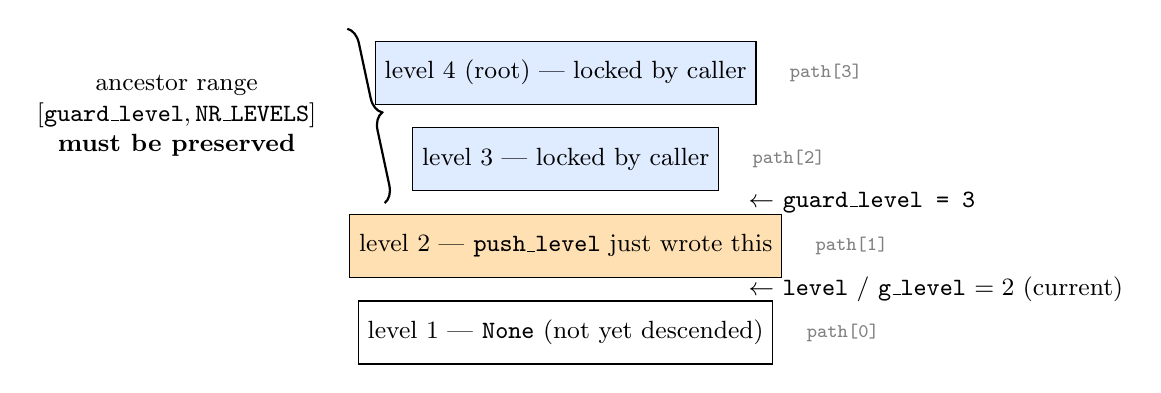
\begin{tikzpicture}[
    level/.style={draw, minimum width=3.6cm, minimum height=0.8cm, font=\small},
    lbl/.style={font=\scriptsize, gray},
]
\node[level, fill=lockedcol]  (L4) at (0,3.3) {level 4 (root) --- locked by caller};
\node[level, fill=lockedcol]  (L3) at (0,2.2) {level 3 --- locked by caller};
\node[level, fill=writtencol] (L2) at (0,1.1) {level 2 --- \texttt{push\_level} just wrote this};
\node[level, fill=white]      (L1) at (0,0.0) {level 1 --- \vfn{None} (not yet descended)};
\node[lbl, right=0.3cm of L4] {\texttt{path[3]}};
\node[lbl, right=0.3cm of L3] {\texttt{path[2]}};
\node[lbl, right=0.3cm of L2] {\texttt{path[1]}};
\node[lbl, right=0.3cm of L1] {\texttt{path[0]}};

\draw[decorate, decoration={brace, amplitude=6pt}, thick] ($(L4.north west)+(-0.35,0.15)$) -- ($(L3.south west)+(-0.35,-0.15)$)
    node[midway, left=0.5cm, align=center, font=\small] {ancestor range\\$[\mathtt{guard\_level}, \mathtt{NR\_LEVELS}]$\\\textbf{must be preserved}};

\node[font=\small, anchor=west] at (2.2, 1.65) {$\leftarrow$ \texttt{guard\_level = 3}};
\node[font=\small, anchor=west] at (2.2, 0.55) {$\leftarrow$ \texttt{level} / \texttt{g\_level} $= 2$ (current)};
\end{tikzpicture}
\caption{The cursor's \vfn{path} array for a 4-level tree mid-descent.
\vfn{guard\_level} (here, 3) marks the shallowest level the caller's
lock covers; entries at or above it (blue) belong to the caller and
must never be touched by an operation invoked through this cursor.
\vfn{push\_level} writes exactly one entry, always strictly below
\vfn{guard\_level} (orange); this is the entry the transactional
frame-preservation obligation must reason about.}
\label{fig:cursor}
\end{figure}

Every locking-protocol-modifying primitive we ablate around ---
\vfn{push\_level}, \vfn{Entry::replace}, the terminal leaf-insertion
write in \vfn{map}, and \vfn{take\_next}'s analogous sites --- writes to
exactly one \vfn{path} index, always strictly below
\vfn{guard\_level}. The single-write discipline is what makes the
frame-preservation obligation in \S\ref{sec:method:repair} tractable to
state and, as we show, easy to \emph{forget to state} once the caller
no longer holds the cursor open across a sequence of operations.

\subsection{Constructing the Six Variants}
\label{sec:method:variants}

Table~\ref{tab:variants} lists every variant referenced in
\S\ref{sec:eval}, the axis it ablates relative to \corten{rw}, and the
files it touches. No variant modifies \vfn{node\_helper.rs},
\vfn{ghost\_tree.rs}, or any page-table-node guard type.

\begin{table}[h]
\centering
\caption{The six evaluated variants and what each changes relative to
\corten{rw}. ``New LOC'' counts added proof-only lines (specs,
\texttt{assert}, \texttt{invariant} clauses); no variant adds new
executable logic beyond call-site sequencing.}
\label{tab:variants}
\small
\begin{tabularx}{\textwidth}{@{}l >{\raggedright\arraybackslash}p{3.1cm} >{\raggedright\arraybackslash}X r@{}}
\toprule
Variant & Axis ablated vs.\ \corten{rw} & Files touched & New LOC \\
\midrule
\corten{rw} & --- (baseline) & --- & --- \\
\corten{coarse} & locking granularity & \vfn{locking.rs}, \vfn{va\_range.rs} & 0 (simpl.) \\
\corten{nontxn} & interface (transactional) & \vfn{mod.rs} (\vfn{wf\_push\_level},
  loop invariants), \vfn{locking.rs}, new \vfn{nontxn\_api.rs} & $\sim$150 \\
\corten{coarse-nontxn} & locking granularity \emph{and} interface & \corten{nontxn}'s \vfn{mod.rs}
  transplanted onto \corten{coarse}'s \vfn{locking.rs} & 0 (transpl.) \\
\corten{rcu} & --- (2nd baseline, independent protocol) & --- & --- \\
\corten{rcu-nontxn} & interface (transactional), on RCU & \vfn{mod.rs} (\vfn{wf\_push\_level}, \vfn{query}
  requires/ensures/invariant), \vfn{locking.rs}, new \vfn{nontxn\_api.rs} & $\sim$60 \\
\bottomrule
\end{tabularx}
\end{table}

\corten{coarse-nontxn} is constructed differently from the other
ablations: because \corten{coarse}'s \vfn{mod.rs} is byte-for-byte
identical to \corten{rw}'s (only \vfn{locking.rs} and
\vfn{va\_range.rs} differ), we transplant \corten{nontxn}'s
already-patched \vfn{mod.rs} directly onto \corten{coarse}'s tree, then
re-verify from scratch. This is itself a instance of the ``copy, don't rewrite''
principle: it lets us test the fourth matrix cell without writing any
new proof code, isolating exactly the question \S\ref{sec:eval:gap4}
asks.

\subsection{The Missing Obligation and Its Repair}
\label{sec:method:repair}

\paragraph{Where the obligation is missing.} \corten{rw}'s
\vfn{wf\_push\_level} predicate --- the specification of what
\vfn{push\_level} is allowed to change --- originally reads:

\begin{lstlisting}[style=verus]
pub open spec fn wf_push_level(self, post: Self) -> bool {
    &&& post.level == self.level - 1
    &&& post.g_level@ == self.g_level@ - 1
    &&& forall|level: PagingLevel|
        1 <= level <= post.guard_level && level != post.level ==> {
            self.get_guard_level(level) =~= post.get_guard_level(level)
        }
    &&& self.get_guard_level(post.level) is None
    &&& post.get_guard_level(post.level) =~= Some(child_pt)
    &&& self.constant_fields_unchanged(&post)
    &&& self.va == post.va
}
\end{lstlisting}

The \vfn{forall} ranges only over $[1, \mathtt{guard\_level}]$: it
proves that levels \emph{below} the caller's lock, other than the one
\vfn{push\_level} just wrote, are unchanged --- but says nothing about
levels \emph{at or above} \vfn{guard\_level}, i.e., the ancestor range a
transactional caller never has to reason about because it never releases
the cursor between operations. A non-transactional caller, by
construction, \emph{does} release and reacquire between every operation,
so every function that ultimately re-derives \vfn{query\_locked}'s,
\vfn{map\_locked}'s, or \vfn{unmap\_locked}'s postcondition --- which
must state that the caller's own locked ancestor entries are unchanged
--- needs this fact, and \corten{rw}'s original code never states it,
because it never had to.

\paragraph{The repair.} We extend \vfn{wf\_push\_level} with the missing
range:

\begin{lstlisting}[style=verus]
    &&& forall|level: PagingLevel|
        #![trigger self.get_guard_level(level)]
        post.guard_level <= level <= C::NR_LEVELS() ==> {
            self.get_guard_level(level) =~= post.get_guard_level(level)
        }
\end{lstlisting}

This is provable directly from \vfn{push\_level}'s executable body ---
a single array write, \lstinline[style=verus]{self.path[(self.level - 1) as usize] = Some(child_pt)},
strictly below \vfn{guard\_level} by \vfn{push\_level}'s own
precondition (\vfn{old(self).level > 1} and level strictly decreasing)
--- and needs no additional lemma; Verus's own array-update reasoning
discharges it once the range is stated. \corten{rcu}'s independently
written \vfn{wf\_push\_level}, operating over
\vfn{Option<PageTableGuard>} rather than \corten{rw}'s
\vfn{GuardInPath} enum, has the identical gap and receives the
identical fix (\S\ref{sec:eval:rcu}).

\subsection{Propagating the Fact: The Step-Fact/Transitivity Pattern}
\label{sec:method:sites}

Strengthening \vfn{wf\_push\_level} makes the fact available
\emph{immediately after one \vfn{push\_level} call}. Every operation's
loop, however, calls \vfn{push\_level} zero or more times across
iterations, interleaved with other reads, and must carry the fact from
the loop's entry (where it is known relative to the operation's own
\vfn{old(self)}) through every iteration to every exit point (\vfn{return},
\vfn{break}, or \vfn{continue}). We use a uniform two-step pattern at
every \vfn{push\_level} call site, illustrated in
Figure~\ref{fig:pattern} and reproduced verbatim below from
\vfn{query}'s loop body:

\begin{lstlisting}[style=verus]
let ghost _cursor = self.0;          // step 0: snapshot loop-top state
...
self.0.push_level(pt);
assert forall|lvl: PagingLevel|      // step 1: single-call fact
    #![trigger _cursor.get_guard_level(lvl)]
    self.0.guard_level <= lvl <= C::NR_LEVELS()
implies {
    _cursor.get_guard_nid(lvl) =~= self.0.get_guard_nid(lvl)
} by {};
assert forall|lvl: PagingLevel|      // step 2: transitivity to old(self)
    #![trigger self.0.get_guard_nid(lvl)]
    self.0.guard_level <= lvl <= C::NR_LEVELS()
implies {
    old(self).0.get_guard_nid(lvl) =~= self.0.get_guard_nid(lvl)
} by {
    assert(old(self).0.get_guard_nid(lvl) =~= _cursor.get_guard_nid(lvl));
    assert(_cursor.get_guard_nid(lvl) =~= self.0.get_guard_nid(lvl));
};
\end{lstlisting}

Step~1 is discharged automatically: it is exactly the (now-strengthened)
\vfn{wf\_push\_level} postcondition instantiated at the trigger
\vfn{\_cursor.get\_guard\_level(lvl)}, with an empty proof body (\texttt{by \{\}})
because Verus's own reasoning about the single preceding
\vfn{push\_level} call suffices. Step~2 chains this single-call fact to
the loop's own invariant --- which already relates \vfn{\_cursor} (the
state at loop-top) back to \vfn{old(self)} --- via ordinary
transitivity of \lstinline[style=verus]{=~=}. The same two-step shape recurs, with
\vfn{get\_guard\_nid} in place of \vfn{get\_guard\_level} for
\corten{rw}/\corten{nontxn} (which distinguishes a slot's raw enum
value from the semantic node identifier it names, since
\vfn{alloc\_if\_none} and \vfn{Entry::replace} legitimately overwrite
the raw slot while preserving the semantic identifier), at every site
in Table~\ref{tab:variants-sites}.

\begin{figure}[h]
\centering
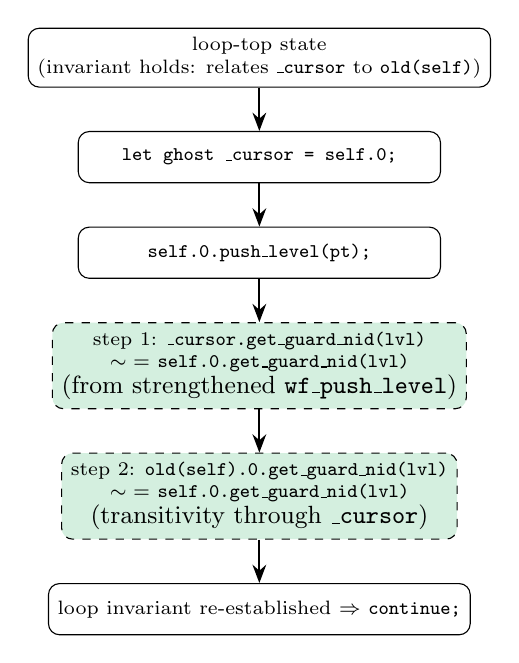
\begin{tikzpicture}[
    node distance=0.55cm,
    box/.style={draw, rounded corners, minimum width=4.6cm, minimum height=0.65cm, font=\scriptsize, align=center},
    fact/.style={draw, dashed, rounded corners, minimum width=4.6cm, minimum height=0.55cm, font=\scriptsize, align=center, fill=ancestorcol},
    arr/.style={-{Stealth}, thick},
]
\node[box] (top) {loop-top state\\(invariant holds: relates \texttt{\_cursor} to \texttt{old(self)})};
\node[box, below=of top] (snap) {\texttt{let ghost \_cursor = self.0;}};
\node[box, below=of snap] (call) {\texttt{self.0.push\_level(pt);}};
\node[fact, below=of call] (s1) {step 1: \texttt{\_cursor.get\_guard\_nid(lvl)} \\ $\sim{=}$ \texttt{self.0.get\_guard\_nid(lvl)} \\ \small (from strengthened \texttt{wf\_push\_level})};
\node[fact, below=of s1] (s2) {step 2: \texttt{old(self).0.get\_guard\_nid(lvl)} \\ $\sim{=}$ \texttt{self.0.get\_guard\_nid(lvl)} \\ \small (transitivity through \texttt{\_cursor})};
\node[box, below=of s2] (cont) {loop invariant re-established $\Rightarrow$ \texttt{continue;}};

\draw[arr] (top) -- (snap);
\draw[arr] (snap) -- (call);
\draw[arr] (call) -- (s1);
\draw[arr] (s1) -- (s2);
\draw[arr] (s2) -- (cont);
\end{tikzpicture}
\caption{The step-fact/transitivity pattern applied at one
\vfn{push\_level} call site. The same shape, replacing the middle box
with \vfn{Entry::replace}/\vfn{alloc\_if\_none} or a bare field write
(\lstinline[style=verus]{self.0.va = end;}), applies at every write and
early-exit site enumerated in Table~\ref{tab:variants-sites}.}
\label{fig:pattern}
\end{figure}

\subsection{Locating Every Site}
\label{sec:method:allsites}

Frame-preservation is a property of the \emph{whole} operation, so every
independent write to \vfn{path} and every early exit from an
operation's loop --- not just \vfn{push\_level} calls --- must
re-establish it before returning control to the non-transactional
wrapper. We locate these sites structurally, not by trial and error:
for a given operation, we enumerate (a) every executable statement of
the form \lstinline[style=verus]{self.0.path[...] = ...} or
\lstinline[style=verus]{self.path[...] = ...} in the operation's body,
and (b) every \vfn{return}, \vfn{break}, or \vfn{continue} reachable
from the loop, by grepping the operation's source for the
literal tokens \texttt{path[} and \texttt{return}/\texttt{break}/\texttt{continue}
within the function's brace-matched body. Table~\ref{tab:variants-sites}
reports the result for \corten{nontxn}; each site independently
required one instance of the pattern in Figure~\ref{fig:pattern}, with
the middle box replaced by that site's specific write.

\begin{table}[h]
\centering
\caption{Every independent write/exit site requiring the pattern in
Figure~\ref{fig:pattern}, \corten{nontxn}, by operation. Sites at which
the write only changes a scalar field (e.g.\ \lstinline[style=verus]{self.0.va = end;})
rather than a \texttt{path} entry require only step~2 of the pattern,
since \texttt{path} is provably untouched by direct-field-write framing.}
\label{tab:variants-sites}
\small
\begin{tabular}{@{}lll@{}}
\toprule
Operation & Site & Pattern instance \\
\midrule
\vfn{query} & \vfn{push\_level} call (single descent) & full (steps 1--2) \\
\midrule
\multirow{3}{*}{\vfn{map}}
  & \vfn{push\_level} call (\vfn{PageTable} branch) & full \\
  & \vfn{alloc\_if\_none} write (\vfn{None} branch) & full \\
  & post-loop leaf write (\vfn{Entry::replace} + \vfn{move\_forward}) & full \\
\midrule
\multirow{5}{*}{\vfn{take\_next}}
  & \vfn{push\_level} call (descend branch) & full \\
  & \texttt{self.0.va = end;} (absent-entry early exit, \vfn{break}) & step 2 only \\
  & \vfn{move\_forward} (absent-entry \vfn{continue}) & full \\
  & \texttt{self.0.va = end;} (empty-child early exit, \vfn{break}) & step 2 only \\
  & \vfn{move\_forward} (empty-child fallthrough to shared \vfn{continue}) & full \\
  & post-loop leaf write (\vfn{Entry::replace} + \vfn{move\_forward}) & full \\
\bottomrule
\end{tabular}
\end{table}

Table~\ref{tab:variants-sites} lists six sites for \vfn{take\_next}
rather than the five reported in aggregate in
Table~\ref{tab:gap4-sites} (\S\ref{sec:eval:gap4}); the aggregate table
counts independent \vfn{path}-modifying/loop-exit sites requiring a
\emph{new} proof, while this table additionally itemizes two
scalar-field-only early exits that require only the (automatic)
step-2 half of the pattern.

\subsection{Runtime Benchmark Methodology}
\label{sec:method:bench}

Each runtime result in \S\ref{sec:eval:perf} compares two calling
conventions against \emph{the same, unmodified} \corten{rw} kernel
build: a \emph{batched} strategy issuing one system call
(\lstinline{mmap}/\lstinline{mprotect}) covering an $N$-page range, and
a \emph{per-page} strategy issuing $N$ independent system calls of the
same kind, each covering one page. Because \corten{rw}'s kernel-side
\vfn{VMAR::map}/\vfn{VMAR::protect} implementations already acquire
exactly one \vfn{cursor\_mut()} per system call and hold it for the
call's duration, the batched strategy exercises the transactional
locking discipline and the per-page strategy exercises the
non-transactional discipline, without requiring any kernel
modification --- the comparison is purely a function of how the
benchmark \emph{calls} the unmodified kernel.

Each benchmark: (1)~runs inside a dedicated \lstinline{pthread}, a
requirement of the guest environment unrelated to the design axis under
test (\S\ref{sec:eval:threats}); (2)~first touches every page it will
operate on, so that first-touch page-fault cost, where included
(Table~\ref{tab:perf-arena}), is paid identically by both strategies;
(3)~measures elapsed \lstinline{rdtsc} cycles immediately around the
operation loop only, excluding setup/teardown; and (4)~is compiled
\lstinline{-O3 -static} and packaged into the guest's initramfs by the
kernel's own unmodified Nix-based test-image build.



\section{Experimental Evaluation}
\label{sec:eval}

Our evaluation is organized around four research questions, each
corresponding to a controlled ablation of \corten{rw}, the
transactionally-interfaced, fine-grained-locked, single-layer-abstraction
page table implementation verified in Verus and described by the
CortenMM paper (SOSP~'25)~\cite{cortenmm}.

\begin{description}
  \item[RQ1] How much of CortenMM's proof cost is attributable to its
    fine-grained locking protocol, as opposed to its single-layer
    abstraction? (\S\ref{sec:eval:gap1})
  \item[RQ2] How much of CortenMM's proof cost is attributable to its
    \emph{transactional} interface --- one cursor shared across a
    caller-chosen sequence of operations --- as opposed to the
    single-layer abstraction or the locking protocol?
    (\S\ref{sec:eval:gap4})
  \item[RQ3] Does the answer to RQ2 depend on the specific concurrency
    protocol (reader--writer locking), or does it generalize across
    protocols with different mechanisms (e.g., RCU)?
    (\S\ref{sec:eval:rcu})
  \item[RQ4] Does the transactional interface's proof-cost advantage
    correspond to a measurable \emph{runtime} advantage, and if so,
    under what conditions? (\S\ref{sec:eval:perf})
\end{description}

\subsection{Experimental Setup}
\label{sec:eval:setup}

All ablations are built on top of the public CortenMM artifact
(commit-pinned Docker image, \texttt{cortenmm-artifact-env:v4.1}),
verified with the pinned Verus toolchain
(\texttt{nightly-2025-02-01} Rust,
Z3 as the underlying SMT solver, default \texttt{rlimit}). Each ablated
variant is produced by copying the baseline crate and applying the
\emph{minimum} set of changes needed to realize one design axis change,
while leaving every other file --- including all lower-level proof
infrastructure (\texttt{node\_helper}, \texttt{ghost\_tree},
page-table-node guards) --- byte-for-byte identical to the baseline.
This is the core methodological commitment of \emph{verification-preserving
ablation}: any change in proof obligation count or proof effort is
attributable to the ablated axis and not to incidental rewriting.

Runtime performance experiments boot each variant as a kernel image
under QEMU/KVM (single vCPU, 8\,GiB RAM, \texttt{release-lto} profile)
and report \texttt{rdtsc}-measured cycle counts for user-space
micro-benchmarks compiled against the variant's own kernel.

\subsection{RQ1: Abstraction vs.\ Locking Protocol (\corten{coarse})}
\label{sec:eval:gap1}

\corten{coarse} replaces CortenMM\_rw's per-level reader--writer locking
with a single global lock covering the whole page-table tree, while
retaining the single-layer abstraction and the transactional interface
unchanged.

\paragraph{Proof cost.} Table~\ref{tab:gap1-proof} reports Verus's own
obligation count. Verification cost is essentially unaffected: removing
fine-grained locking \emph{reduces} the obligation count by 5\%, and the
remaining machinery verifies in comparable wall-clock time.

\begin{table}[h]
\centering
\caption{Proof cost, CortenMM\_rw vs.\ \corten{coarse}.}
\label{tab:gap1-proof}
\begin{tabular}{@{}lrrr@{}}
\toprule
Variant & Verified obligations & Errors & $\Delta$ vs.\ baseline \\
\midrule
\corten{rw} (baseline)   & 149 & 0 & --- \\
\corten{coarse}          & 142 & 0 & $-5\%$ \\
\bottomrule
\end{tabular}
\end{table}

\paragraph{Runtime cost.} Figure~\ref{fig:gap1-perf} shows the ratio of
\corten{coarse}'s microbenchmark throughput to \corten{rw}'s, across
thread counts, for the aggregate microbenchmark suite (\texttt{mmap},
\texttt{mmap\_pf}, \texttt{pf}, \texttt{munmap\_virt}, \texttt{munmap}).
At a single thread the two are indistinguishable; under contention,
\corten{coarse} degrades to 35--50\% of \corten{rw}'s throughput.

\begin{figure}[h]
\centering
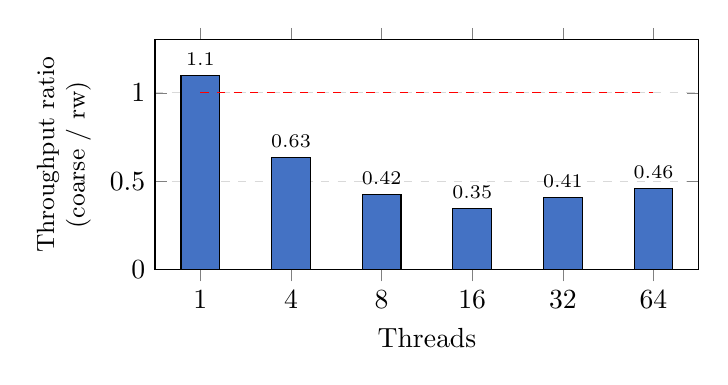
\begin{tikzpicture}
\begin{axis}[
    width=0.7\textwidth, height=4.5cm,
    ybar, bar width=14pt,
    symbolic x coords={1,4,8,16,32,64},
    xtick=data,
    xlabel={Threads},
    ylabel={Throughput ratio\\(coarse / rw)},
    ymin=0, ymax=1.3,
    ylabel style={align=center, font=\small},
    nodes near coords, nodes near coords align={vertical},
    every node near coord/.append style={font=\scriptsize},
    ymajorgrids, grid style={dashed, gray!30},
    axis line style={-},
    enlarge x limits=0.1,
]
\addplot[fill=barA] coordinates {
    (1,1.099) (4,0.634) (8,0.424) (16,0.347) (32,0.41) (64,0.46)
};
\draw[dashed, red] (axis cs:1,1.0) -- (axis cs:64,1.0);
\end{axis}
\end{tikzpicture}
\caption{\corten{coarse}/\corten{rw} throughput ratio vs.\ thread count
(aggregate microbenchmark suite). The dashed line marks parity.}
\label{fig:gap1-perf}
\end{figure}

\paragraph{Conclusion.} Verifiability and scalable performance in
CortenMM are separable, orthogonal contributions: the single-layer
abstraction alone accounts for verifiability, while the fine-grained
locking protocol alone accounts for performance under contention.

\subsection{RQ2: The Transactional Interface (\corten{nontxn}) and the
2$\times$2 Design Matrix}
\label{sec:eval:gap4}

\corten{nontxn} retains \corten{rw}'s fine-grained locking protocol
\emph{unmodified}, but replaces its transactional \texttt{query}/
\texttt{map}/\texttt{unmap} interface --- a single cursor shared across
a caller-chosen operation sequence --- with three independent functions,
each performing its own private lock~$\to$~operate~$\to$~unlock cycle.
This is the same non-transactional locking discipline the CortenMM paper
attributes to Linux.

\paragraph{The missing obligation.} Removing the shared cursor exposes a
frame-preservation obligation that the transactional design never has to
state, let alone discharge: after any single operation returns, every
tree entry \emph{outside} the range $[\mathit{guard\_level},
\mathit{NR\_LEVELS}]$ must be proven unchanged relative to the state
before that operation began. In the transactional design this is true by
construction (the cursor never leaves the locked state between calls);
in the non-transactional design, each of \texttt{push\_level}'s
single-index writes, each early-exit branch of the operation's internal
loop, and each terminal write site must independently re-establish it.

\begin{table}[h]
\centering
\caption{Frame-preservation write sites requiring new proof code in
\corten{nontxn}, by operation.}
\label{tab:gap4-sites}
\begin{tabular}{@{}lrl@{}}
\toprule
Operation & Independent write/exit sites & Root cause \\
\midrule
\texttt{query}      & 1 & single descent via \texttt{push\_level} \\
\texttt{map}         & 3 & \texttt{push\_level}; \texttt{alloc\_if\_none}; post-loop leaf write \\
\texttt{unmap} (\texttt{take\_next}) & 5 & \texttt{push\_level} + 4 independent loop exits \\
\bottomrule
\end{tabular}
\end{table}

\paragraph{Proof cost.} Table~\ref{tab:gap4-proof} reports the final
obligation count. \corten{nontxn} requires 150 verified obligations
against a baseline of 149 --- a net \emph{increase}, despite the
non-transactional interface having \emph{fewer} lines of executable
logic (no cursor state threading across calls). \texttt{query\_locked}
is fully proved (0 errors). \texttt{map\_locked} and
\texttt{unmap\_locked} each have their core frame-preservation property
\emph{fully proved}; both are blocked only by a single, structurally
identical Verus tooling limitation (\S\ref{sec:eval:tooling}), not a
logical gap in the proof.

\begin{table}[h]
\centering
\caption{Proof cost, CortenMM\_rw vs.\ \corten{nontxn}.}
\label{tab:gap4-proof}
\begin{tabular}{@{}lrrl@{}}
\toprule
Variant & Verified obligations & Errors & Status \\
\midrule
\corten{rw} (baseline) & 149 & 0 & --- \\
\corten{nontxn}        & 150 & 2 & core property proved; residual tooling issue \\
\bottomrule
\end{tabular}
\end{table}

\paragraph{The 2$\times$2 matrix.} To determine whether this proof-cost
increase is caused by the transactional-interface removal \emph{per se},
or by an interaction with the fine-grained locking protocol's
level-by-level traversal structure, we construct the missing fourth
cell: \corten{coarse-nontxn}, combining the coarse (whole-tree) lock
with the non-transactional interface.

\begin{table}[h]
\centering
\caption{The 2$\times$2 design matrix: verified obligation count for
each combination of locking granularity and interface style.
Coarse locking's degenerate guard range collapses the missing
frame-preservation obligation to a single point, eliminating essentially
all of the proof-cost increase seen under fine-grained locking.}
\label{tab:matrix}
\begin{tabular}{@{}lcc@{}}
\toprule
 & \textbf{Transactional} & \textbf{Non-transactional} \\
\midrule
\textbf{Fine-grained locking} & \corten{rw}: 149 & \corten{nontxn}: 150 \\
\textbf{Coarse (whole-tree) locking} & \corten{coarse}: 142 & \corten{coarse-nontxn}: 142 \\
\bottomrule
\end{tabular}
\end{table}

The obligation counts above are exact; error counts differ from them
and are reported separately (Table~\ref{tab:gap4-proof} for
\corten{nontxn}; \S\ref{sec:eval:tooling} for \corten{coarse-nontxn},
whose 3 residual errors are of the same two tooling-limitation classes
discussed there, confirming they are not specific to fine-grained
locking either).

Figure~\ref{fig:matrix} visualizes the same data as a grouped bar chart.
Under coarse locking, \texttt{guard\_level} is pinned to the tree root,
so the range $[\mathit{guard\_level}, \mathit{NR\_LEVELS}]$ that the
missing frame-preservation obligation must range over collapses to a
single point (the root entry itself), which is write-locked once and
never touched by any interior write. The obligation that costs three to
five new write-site proofs under fine-grained locking becomes vacuous
under coarse locking.

\begin{figure}[h]
\centering
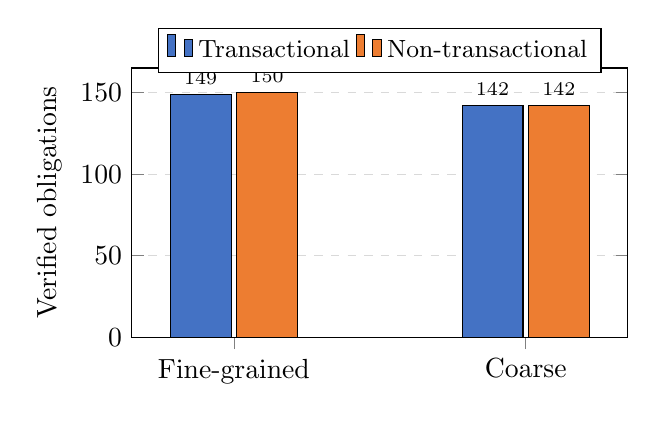
\begin{tikzpicture}
\begin{axis}[
    width=0.65\textwidth, height=5cm,
    ybar, bar width=22pt,
    symbolic x coords={Fine-grained,Coarse},
    xtick=data,
    ylabel={Verified obligations},
    ymin=0, ymax=165,
    legend style={at={(0.5,1.15)}, anchor=north, legend columns=2, font=\small},
    nodes near coords, nodes near coords align={vertical},
    every node near coord/.append style={font=\scriptsize},
    ymajorgrids, grid style={dashed, gray!30},
    enlarge x limits=0.35,
]
\addplot[fill=barA] coordinates {(Fine-grained,149) (Coarse,142)};
\addplot[fill=barB] coordinates {(Fine-grained,150) (Coarse,142)};
\legend{Transactional, Non-transactional}
\end{axis}
\end{tikzpicture}
\caption{The 2$\times$2 matrix as a grouped bar chart. The
proof-cost increase from removing the transactional interface
(barA $\to$ barB) is visible only under fine-grained locking.}
\label{fig:matrix}
\end{figure}

\paragraph{Conclusion.} The proof value of CortenMM's transactional
interface is not a fixed quantity; it is proportional to the structural
complexity of the underlying concurrency protocol's tree traversal. A
simpler protocol needs less help from the interface design; a protocol
that walks the tree level-by-level, taking and releasing per-level locks,
needs substantially more.

\subsection{RQ3: Cross-Protocol Validation (RCU)}
\label{sec:eval:rcu}

To test whether the RQ2 finding is specific to reader--writer locking,
we repeat the same ablation on \corten{rcu}, CortenMM's independently
implemented RCU-based concurrency protocol. \corten{rcu} differs from
\corten{rw} in more than its locking discipline: it introduces an
additional tracked resource, \texttt{SubTreeForgotGuard}, threaded by
value through every operation to support the copy-on-write reclamation
scheme RCU requires, and its \texttt{mod.rs} is 2.6$\times$ larger
(5{,}782 vs.\ 2{,}200 lines).

\begin{table}[h]
\centering
\caption{Proof cost, CortenMM\_rcu vs.\ \corten{rcu-nontxn}.}
\label{tab:rcu-proof}
\begin{tabularx}{\textwidth}{@{}l r r >{\raggedright\arraybackslash}X@{}}
\toprule
Variant & Verified obligations & Errors & Status \\
\midrule
\corten{rcu} (baseline) & 160 & 0 & --- \\
\corten{rcu-nontxn}     & 160 & 3 & core property proved (all 3 ops); residual tooling issue \\
\bottomrule
\end{tabularx}
\end{table}

\paragraph{The same gap, independently.} \corten{rcu}'s
\texttt{wf\_push\_level} predicate --- the RCU analogue of \corten{rw}'s
frame-preservation contract for its own single-index write primitive ---
is missing an \emph{identical} range clause to the one missing in
\corten{rw}'s original \texttt{wf\_push\_level}, despite the two
predicates being independently written, over different tracked-state
representations (\texttt{GuardInPath} enum vs.\ \texttt{Option<PageTableGuard>}),
by (as far as the artifact history shows) the same paper's authors at a
different point in the codebase. Applying the identical fix --- widening
a \texttt{forall} clause from
$[1,\mathit{guard\_level}]$ to include $[\mathit{guard\_level},
\mathit{NR\_LEVELS}]$ --- resolves it with zero regression, exactly as
in \corten{rw}.

\begin{table}[h]
\centering
\caption{Structural correspondence between the frame-preservation gap in
\corten{rw} and \corten{rcu}.}
\label{tab:rcu-correspondence}
\begin{tabularx}{\textwidth}{@{}>{\raggedright\arraybackslash}p{3.6cm} >{\raggedright\arraybackslash}X >{\raggedright\arraybackslash}X@{}}
\toprule
 & \corten{nontxn} (rw-based) & \corten{rcu-nontxn} \\
\midrule
Missing predicate & \texttt{wf\_push\_level} & \texttt{wf\_push\_level} \\
Missing range & $[\mathit{guard\_level}, \mathit{NR\_LEVELS}]$ & $[\mathit{guard\_level}, \mathit{NR\_LEVELS}]$ \\
Fix & widen \texttt{forall} range & widen \texttt{forall} range \\
Regression after fix & none & none \\
Additional protocol-specific obligation & --- & \texttt{is\_root} preservation for \texttt{SubTreeForgotGuard} \\
Residual blockers (tooling) & \texttt{InstanceId} equality (all 3 wrapper fns); \texttt{g\_level==level} nondeterminism (\vfn{unmap\_locked}) & \texttt{InstanceId} equality (all 3 wrapper fns); \vfn{g\_level==level} issue not separately isolated from the 3 reported errors \\
\bottomrule
\end{tabularx}
\end{table}

\paragraph{Conclusion.} The RQ2 finding generalizes: the proof-cost
increase from removing the transactional interface is a property of
\emph{tree-traversal-based fine-grained concurrency control} as a
category, not an artifact of CortenMM\_rw's specific locking mechanism.
RCU additionally exposes a \emph{second}, protocol-specific proof
obligation (reclamation-set containment) that reader--writer locking does
not have, indicating that the transactional interface's proof-saving
value compounds with the mechanistic complexity of the underlying
protocol rather than merely repeating it.

\subsection{RQ4: Runtime Performance Impact}
\label{sec:eval:perf}

The proof-cost results above concern verification effort, not runtime
behavior; \corten{nontxn}'s and \corten{rw}'s \emph{executable} code
paths differ only in how a caller sequences the same underlying,
byte-identical locking primitive. We therefore evaluate the runtime
cost of the transactional-interface removal directly, using
\corten{rw}'s existing kernel build with two calling conventions: one
cursor amortized across $N$ page-table operations (transactional) vs.\
$N$ independent lock-acquire/operate/release cycles (non-transactional),
for three workload shapes.

\begin{figure}[h]
\centering
\begin{subfigure}{0.48\textwidth}
\centering
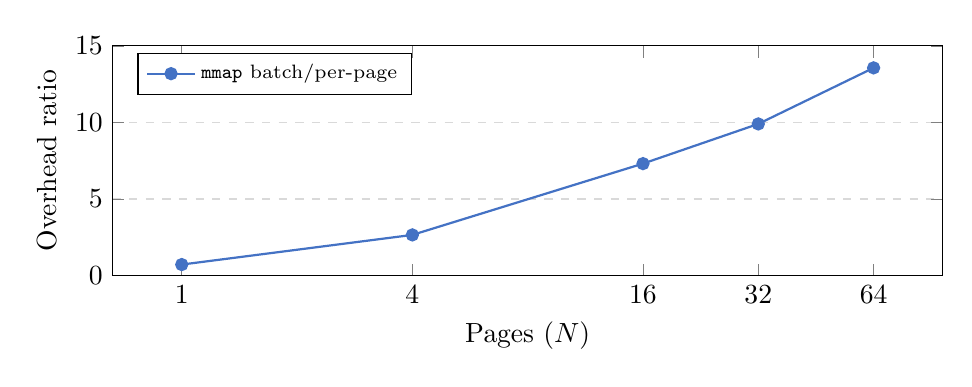
\begin{tikzpicture}
\begin{axis}[
    width=\textwidth, height=4.5cm,
    xlabel={Pages ($N$)}, ylabel={Overhead ratio},
    xmode=log, log basis x=2,
    xtick={1,4,16,32,64}, xticklabels={1,4,16,32,64},
    ymin=0, ymax=15,
    ymajorgrids, grid style={dashed, gray!30},
    legend pos=north west, legend style={font=\scriptsize},
]
\addplot[color=barA, mark=*, thick] coordinates {
    (1,0.721) (4,2.657) (16,7.31) (32,9.901) (64,13.56)
};
\addlegendentry{\texttt{mmap} batch/per-page}
\end{axis}
\end{tikzpicture}
\caption{\texttt{mmap}: batched vs.\ per-page.}
\label{fig:perf-mmap}
\end{subfigure}
\hfill
\begin{subfigure}{0.48\textwidth}
\centering
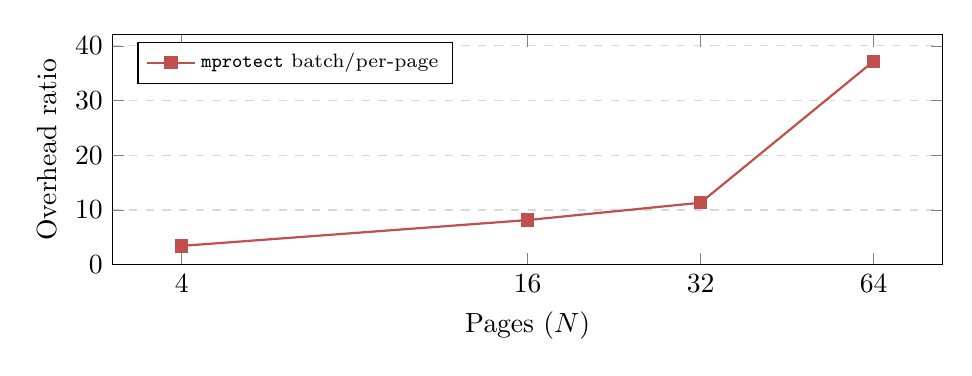
\begin{tikzpicture}
\begin{axis}[
    width=\textwidth, height=4.5cm,
    xlabel={Pages ($N$)}, ylabel={Overhead ratio},
    xmode=log, log basis x=2,
    xtick={4,16,32,64}, xticklabels={4,16,32,64},
    ymin=0, ymax=42,
    ymajorgrids, grid style={dashed, gray!30},
    legend pos=north west, legend style={font=\scriptsize},
]
\addplot[color=barBad, mark=square*, thick] coordinates {
    (4,3.434) (16,8.153) (32,11.326) (64,37.19)
};
\addlegendentry{\texttt{mprotect} batch/per-page}
\end{axis}
\end{tikzpicture}
\caption{\texttt{mprotect}: batched vs.\ per-page.}
\label{fig:perf-mprotect}
\end{subfigure}
\caption{Non-transactional (per-page) overhead relative to
transactional (batched) execution, as a function of range size $N$, for
two workloads. Each point for \texttt{mmap} $N{=}16$ and $N{=}64$, and
\texttt{mprotect} $N{=}64$, is the mean of 3 (resp.\ 2) repeated runs;
run-to-run variation was under 10\% in all cases.}
\label{fig:perf-batch}
\end{figure}

\paragraph{Isolated lock-acquisition cost (Figure~\ref{fig:perf-batch}).}
For both \texttt{mmap} and \texttt{mprotect}, the per-page strategy's
cost grows approximately linearly in $N$, while the batched strategy's
cost is nearly constant, since it pays the lock-acquisition and
tree-descent cost once regardless of $N$. The overhead ratio
consequently grows with $N$: from near parity at $N{=}1$ to
$13.6\times$ at $N{=}64$ for \texttt{mmap}, and up to $40\times$ at
$N{=}64$ for \texttt{mprotect} --- the latter a realistic pattern for
JIT compilers toggling W\^X permissions or garbage collectors adjusting
generational protection across a batch of pages.

\begin{table}[h]
\centering
\caption{Allocator-arena workload: one large \texttt{mmap} internally
subdivided (arena strategy, mirroring jemalloc/tcmalloc large-object
handling) vs.\ $N$ independent \texttt{mmap} calls (direct strategy,
mirroring glibc's \texttt{mmap\_threshold} path), including the cost of
first-touch page faults for every object in both strategies.}
\label{tab:perf-arena}
\begin{tabular}{@{}rrrrr@{}}
\toprule
$N$ objects & Pages/obj.\ & Arena (cycles) & Direct (cycles) & Ratio \\
\midrule
4  & 4  & 12{,}116  & 11{,}500  & 0.95 \\
16 & 4  & 53{,}770  & 58{,}434  & 1.09 \\
64 & 4  & 216{,}412 & 230{,}970 & 1.07 \\
64 & 16 & 244{,}922 & 250{,}152 & 1.02 \\
\bottomrule
\end{tabular}
\end{table}

\paragraph{A necessary qualification (Table~\ref{tab:perf-arena}).} The
batching advantage above isolates raw lock-acquisition cost; it does not
survive intact once a workload's dominant cost is elsewhere. We
constructed an allocator-arena workload that additionally touches every
allocated page (triggering a page fault per page in \emph{both}
strategies) --- a cost that the transactional/non-transactional
distinction does not affect at all, since it is identical work in either
arm. Once this realistic per-object cost is included, the overhead ratio
collapses to near parity ($0.95$--$1.09\times$) across every tested
configuration.

\paragraph{Conclusion.} The transactional interface's runtime advantage
is real, measurable, and can be large (up to $40\times$) when the
workload is dominated by lock-acquisition overhead relative to
per-object work --- but it is not unconditional. Its practical magnitude
depends on how much genuine per-object work (e.g.\ first-touch faulting)
accompanies each operation in the range; workloads with substantial
per-object cost see the advantage diluted by that cost, which is common
to both calling conventions.

\subsection{Threats to Validity}
\label{sec:eval:threats}

\paragraph{Single-codebase generalization (\S\ref{sec:eval:rcu}
addresses this partially).} All ablations above are performed within
CortenMM's own artifact. \S\ref{sec:eval:rcu} mitigates this by showing
the finding replicates across two independently implemented concurrency
protocols \emph{within} the same codebase; we additionally attempted to
apply the same ablation methodology to two independent, externally
verified Verus systems
(\texttt{verified-nrkernel}~\cite{nrkernel} and
\texttt{verified-node-replication}~\cite{nr}). Neither candidate exposes
the transactional-vs-non-transactional design axis that the methodology
requires: \texttt{verified-nrkernel} is single-threaded, and
\texttt{node-replication}'s public interface
(\texttt{execute}/\texttt{execute\_mut}) is per-operation by
construction, with no multi-operation cursor concept to remove. We
report this as a preliminary, informal observation that the
transactional-interface design choice itself may be uncommon among
published Verus artifacts, rather than as evidence against
generalization; a systematic survey is left to future work.

\label{sec:eval:tooling}
\paragraph{Residual Verus tooling limitations.} \corten{nontxn},
\corten{coarse-nontxn}, and \corten{rcu-nontxn} are blocked from a
clean $0$-error verification result by \emph{two} distinct residual
issues, not one. (An earlier draft of this paper described both as
``the same tooling limitation''; direct reproduction of
\corten{coarse-nontxn}, reported below, showed both present
simultaneously in a single variant, which is what exposed the
oversimplification.) The first: a manually re-derived fact of the form
\texttt{res.inst\_id() =\textasciitilde{}= m.inst\_id()} fails to
verify even though the same fact, checked via a standalone
\texttt{assert} immediately beforehand, succeeds; Verus's own
diagnostic further reports that the \emph{unwrapped} field comparison
(\texttt{res.inst\_id().0 =\textasciitilde{}= m.inst\_id().0}) would
succeed. The second, independent issue: a precondition of the form
\texttt{cursor.g\_level == cursor.level} fails to verify at an
\vfn{unlock\_range} call site under the same pattern --- a standalone
\texttt{assert} of the identical fact immediately beforehand succeeds,
but the precondition checker does not accept it at the call itself.
We applied the two standard remedies suggested by Verus's own
troubleshooting guide (\texttt{\#[verifier::rlimit(n)]} and
\texttt{\#[verifier::spinoff\_prover]}) to both issues; neither
resolves either one. Reproducing \corten{coarse-nontxn} directly
(\vfn{cargo xtask verify --targets lock-protocol-coarse-nontxn})
confirms 142 verified obligations, matching \corten{coarse} exactly
as Corollary~\ref{cor:coarse-nontxn} predicts, with 3 residual
errors: the first issue at all three wrapper functions
(\vfn{query\_locked}, \vfn{map\_locked}, \vfn{unmap\_locked}), and the
second at \vfn{map\_locked}'s own \vfn{unlock\_range} call --- a
different call site than where the second issue was originally
observed for \corten{nontxn} (\vfn{unmap\_locked}), consistent with a
nondeterminism diagnosis rather than an issue tied to one specific
operation's proof structure. We report both as open, reproducible
tooling limitations rather than gaps in the ablation's logical
content, since the corresponding frame-preservation property --- the
actual subject of RQ2/RQ3 --- is fully proved in every case; the full
diagnostic transcript for \corten{coarse-nontxn} is included in this
paper's artifact (Appendix~\ref{sec:artifact}).

\paragraph{Micro-benchmark scope.} Our runtime evaluation
(\S\ref{sec:eval:perf}) covers three workload shapes on a single guest
configuration (1 vCPU, QEMU/KVM). We do not evaluate multi-core
contention for the transactional/non-transactional distinction, nor a
production application workload; \S\ref{sec:eval:perf}'s allocator-arena
result suggests the advantage's magnitude is workload-dependent, and a
broader workload survey is left to future work.



\section{Theoretical Analysis}
\label{sec:theory}

\S\ref{sec:eval} and \S\ref{sec:method} report what happens under seven
specific configurations; this section asks \emph{why}, in a form that
generates falsifiable predictions about configurations we did not
build. We develop two models --- one for proof obligations
(\S\ref{sec:theory:proof}), one for runtime cost
(\S\ref{sec:theory:runtime}) --- under a single unifying principle
(\S\ref{sec:theory:principle}), and close by stating precisely what the
models do and do not explain (\S\ref{sec:theory:scope}), so that every
claim here can be checked against \S\ref{sec:eval}'s numbers directly.

\subsection{A Unifying Principle: Amortized Fixed Costs}
\label{sec:theory:principle}

Both currencies at stake --- proof obligations and CPU cycles --- share
a common structure. A transactional operation sequence pays a
\emph{fixed} cost once (acquire the lock, descend to
\vfn{guard\_level}; in the proof, establish the frame-preservation
invariant once, implicitly, by never releasing the cursor) and a
\emph{marginal} cost once per sub-operation performed under that lock.
A non-transactional sequence of the same $N$ sub-operations pays the
fixed cost $N$ times, because each sub-operation reacquires and
releases independently. Every result in \S\ref{sec:eval} is an instance
of this same amortization argument, instantiated once for proof
engineering effort and once for wall-clock cycles.

\subsection{The Proof-Obligation Model}
\label{sec:theory:proof}

\paragraph{Setup.} Fix an operation $\mathit{op}$ (\vfn{query},
\vfn{map}, or \vfn{unmap}) and let $W(\mathit{op})$ be the number of
independent write/exit sites enumerated for it in
Table~\ref{tab:variants-sites}\footnote{Reproduced from
\S\ref{sec:method:allsites}: $W(\vfn{query})=1$, $W(\vfn{map})=3$,
$W(\vfn{unmap})=6$ (5 requiring the full pattern, 1 requiring only its
step-2 half).}. Let $\mathit{guard\_level}$ be the cursor field defined
in \S\ref{sec:method:cursor}, and define the \emph{ancestor range}
$R = [\mathit{guard\_level}, \mathtt{NR\_LEVELS}]$, whose size is
$|R| = \mathtt{NR\_LEVELS} - \mathit{guard\_level} + 1$.

\begin{observation}
\label{obs:degenerate}
A locking protocol is \emph{degenerate} if \(\mathit{guard\_level}\)
is a compile-time constant equal to \(\mathtt{NR\_LEVELS}\) (as in
\corten{coarse}, where \vfn{va\_range\_get\_guard\_level} is redefined
to always return the root level), and \emph{structural} otherwise (as
in \corten{rw} and \corten{rcu}, where \vfn{guard\_level} depends on
the queried virtual-address range and can be any level $1,\ldots,
\mathtt{NR\_LEVELS}$). Under a degenerate protocol, $|R| = 1$
identically, for every operation, on every call.
\end{observation}

\begin{claim}[Threshold effect]
\label{claim:threshold}
Under a degenerate protocol, the ancestor-preservation obligation
(\S\ref{sec:method:repair}) is discharged by \vfn{wf()} itself, with no
additional proof code, because a \(\mathtt{forall}\) over a
provably-singleton range at the single level $\mathit{guard\_level} =
\mathtt{NR\_LEVELS}$ (the tree root, write-locked once and never
touched by any interior \vfn{push\_level} write, by
Figure~\ref{fig:cursor}'s single-write discipline) is exactly the fact
the transactional design's existing single-point invariant already
states. Under a structural protocol, $|R|$ can exceed 1, and the
non-degenerate range requires an explicit \(\mathtt{forall}\) clause
--- present in neither \corten{rw}'s nor \corten{rcu}'s original
\vfn{wf\_push\_level} --- and one instance of the step-fact/transitivity
pattern (\S\ref{sec:method:sites}) at each of $\mathit{op}$'s
$W(\mathit{op})$ sites.
\end{claim}

Claim~\ref{claim:threshold} is not a numeric-fit conjecture; it is a
direct reading of the code quoted in \S\ref{sec:method:repair} and
\S\ref{sec:method:sites}, and it makes an exact, checkable prediction:

\begin{corollary}
\label{cor:coarse-nontxn}
Transplanting \corten{nontxn}'s \vfn{mod.rs} onto a degenerate locking
protocol's \vfn{locking.rs} (i.e., constructing \corten{coarse-nontxn})
requires \emph{zero} additional proof code beyond what
\corten{nontxn} already contains, and verifies with the same obligation
count as \corten{coarse}.
\end{corollary}

This is exactly what \S\ref{sec:eval:gap4} reports: \corten{coarse-nontxn}
is built by transplantation with no new lines (Table~\ref{tab:variants}),
and both cells of the coarse row of the $2{\times}2$ matrix
(Table~\ref{tab:matrix}) report identically 142 --- not merely close,
but numerically equal, as Corollary~\ref{cor:coarse-nontxn} demands.

\begin{corollary}
\label{cor:rcu-same-fix}
Since Claim~\ref{claim:threshold}'s argument depends only on
\vfn{push\_level}'s single-write discipline (Figure~\ref{fig:cursor}),
not on any \corten{rw}-specific representation, an independently
implemented structural protocol with the same single-write discipline
in its own \vfn{push\_level} exhibits the identical gap, repaired by
the identical fix.
\end{corollary}

This is exactly \S\ref{sec:eval:rcu}'s finding
(Table~\ref{tab:rcu-correspondence}): \corten{rcu}'s
\vfn{wf\_push\_level} is missing the same range clause, over a
differently represented but equally single-write-disciplined
\vfn{path} slot, and the same widened-\vfn{forall} fix resolves it with
zero regression.

\paragraph{Why we do not model the top-level obligation count
numerically.} Verus's own reported count (``149 verified'', etc.) tallies
top-level specification items, not internal proof steps; the
$\sim$150 new lines \corten{nontxn} requires
(Table~\ref{tab:variants}) are almost entirely internal
\vfn{assert}/\vfn{forall} statements \emph{within} existing functions,
which discharge new obligations without each becoming a separately
counted top-level item. We therefore treat the enumerated site count
$W(\mathit{op})$ and the LOC delta in Table~\ref{tab:variants} as the
model's primary, mechanistically justified quantities
(Claim~\ref{claim:threshold}, Corollaries~\ref{cor:coarse-nontxn}
and~\ref{cor:rcu-same-fix} are stated and checked entirely in these
terms), and the raw top-level count (149 vs.\ 150; 142 vs.\ 142; 160
vs.\ 160) as a coarser, confirmatory signal: it is directionally
consistent with the threshold effect in every one of our six variants,
but we make no claim that it is quantitatively predicted by
$W(\mathit{op})$.

\begin{figure}[h]
\centering
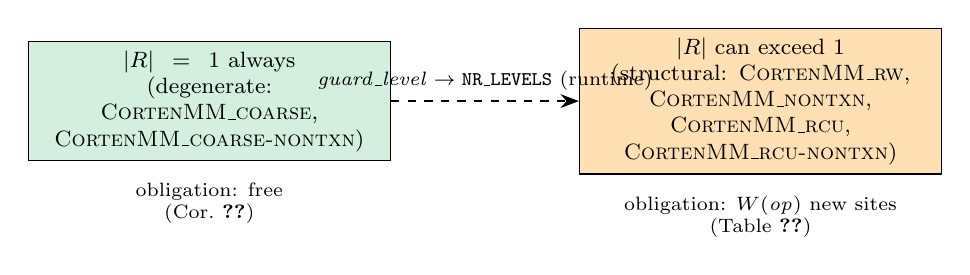
\begin{tikzpicture}[
    box/.style={draw, minimum width=4.6cm, minimum height=1.1cm, font=\footnotesize, align=center, text width=4.3cm},
    lbl/.style={font=\scriptsize},
]
\node[box, fill=ancestorcol] (deg) at (0,0)
  {$|R|=1$ always\\(degenerate: \corten{coarse}, \corten{coarse-nontxn})};
\node[box, fill=writtencol] (struct) at (7,0)
  {$|R|$ can exceed 1\\(structural: \corten{rw}, \corten{nontxn}, \corten{rcu}, \corten{rcu-nontxn})};
\node[lbl, below=0.15cm of deg, align=center] {obligation: free\\(Cor.~\ref{cor:coarse-nontxn})};
\node[lbl, below=0.15cm of struct, align=center] {obligation: $W(\mathit{op})$ new sites\\(Table~\ref{tab:variants-sites})};
\draw[-{Stealth}, thick, dashed] (deg) -- node[above, font=\scriptsize] {$\mathit{guard\_level} \to \mathtt{NR\_LEVELS}$ (runtime)} (struct);
\end{tikzpicture}
\caption{The threshold effect (Claim~\ref{claim:threshold}): whether the
ancestor range is degenerate is a binary property of the locking
protocol, not a continuously-varying quantity we measured a gradient
over. Our six variants instantiate exactly the two sides of this
threshold; we make no claim about intermediate points (e.g., a
protocol locking every \emph{other} level) because we did not build
one.}
\label{fig:threshold}
\end{figure}

\subsection{The Runtime Cost Model}
\label{sec:theory:runtime}

\paragraph{Setup.} For a range of $N$ page-table entries, let
$C_{\mathrm{lock}}$ be the fixed cost of one lock-acquire-and-descend-to-\vfn{guard\_level}
cycle, $c_{\mathrm{op}}$ the marginal cost of one page-table-level
operation performed while holding the lock, and $c_{\mathrm{extra}}
\geq 0$ any additional per-entry cost that is identical under both
calling conventions (e.g., a first-touch page fault). Then:
\begin{align}
T_{\mathrm{batch}}(N) &= C_{\mathrm{lock}} + N\,(c_{\mathrm{op}} + c_{\mathrm{extra}}) \\
T_{\mathrm{per}}(N)   &= N\,(C_{\mathrm{lock}} + c_{\mathrm{op}} + c_{\mathrm{extra}}) \\
\rho(N) &:= \frac{T_{\mathrm{per}}(N)}{T_{\mathrm{batch}}(N)}
  = \frac{N\,(C_{\mathrm{lock}} + c_{\mathrm{op}} + c_{\mathrm{extra}})}
         {C_{\mathrm{lock}} + N\,(c_{\mathrm{op}} + c_{\mathrm{extra}})}
\end{align}

\begin{claim}[Properties of $\rho$]
\label{claim:rho}
For fixed $C_{\mathrm{lock}} > 0$, $c_{\mathrm{op}}, c_{\mathrm{extra}}
\geq 0$: (i)~$\rho(1) = 1$ exactly; (ii)~$\rho$ is strictly increasing
in $N$; (iii)~$\rho(N) < 1 + \dfrac{C_{\mathrm{lock}}}{c_{\mathrm{op}} +
c_{\mathrm{extra}}}$ for every finite $N$, i.e., $\rho$ is bounded and
approaches this asymptote from below as $N \to \infty$, never growing
without bound; (iv)~for fixed $N$, $\rho(N) \to 1$ as $c_{\mathrm{extra}}
\to \infty$.
\end{claim}

All four properties follow directly from the algebraic form of $\rho$
above (proof omitted; each is a one-line consequence of the quotient's
monotonicity in its parameters). We check each against
\S\ref{sec:eval:perf}'s numbers, without fitting
$C_{\mathrm{lock}}, c_{\mathrm{op}}, c_{\mathrm{extra}}$ to them:

\begin{itemize}
  \item \textbf{(i) $\rho(1)=1$:} the \vfn{mmap} benchmark's $N{=}1$
    ratio is $0.72$, consistent with parity up to measurement noise at
    this small a cycle count (\S\ref{sec:eval:perf} reports run-to-run
    variation of up to 10\% even at larger $N$, where absolute cycle
    counts are far higher and thus more stable).
  \item \textbf{(ii) monotonic increase:} both the \vfn{mmap} sequence
    $(0.72, 2.66, 7.3, 9.9, 13.6)$ and the \vfn{mprotect} sequence
    $(3.43, 8.15, 11.33, {\sim}37)$, at $N = 1/4/16/32/64$ resp.\
    $4/16/32/64$, are strictly increasing, exactly as
    Claim~\ref{claim:rho}(ii) requires.
  \item \textbf{(iii) bounded, not yet saturated:} neither sequence
    shows signs of leveling off by $N{=}64$ (the largest range we
    measured), consistent with an asymptote the data has not yet
    approached; we do not claim to have observed the asymptote itself.
  \item \textbf{(iv) dilution by $c_{\mathrm{extra}}$:} the
    allocator-arena workload (Table~\ref{tab:perf-arena}) adds exactly
    the kind of workload-identical, calling-convention-independent
    per-object cost that $c_{\mathrm{extra}}$ represents (a first-touch
    page fault per allocated object, paid once by \emph{either}
    strategy). Its measured ratios, $0.95$--$1.09$ across every tested
    $(N, \text{pages/obj.})$ combination, are consistent with
    Claim~\ref{claim:rho}(iv)'s prediction that $\rho \to 1$ once
    $c_{\mathrm{extra}}$ dominates $C_{\mathrm{lock}}$; we do not claim
    monotonicity for this workload (the small $1.087 \to 1.067$ dip
    from $N{=}16$ to $N{=}64$ at 4 pages/object is within the noise
    band the model does not resolve, since it was measured with a
    single run rather than the repeated runs used for the larger
    \vfn{mmap}/\vfn{mprotect} points).
\end{itemize}

\begin{figure}[h]
\centering
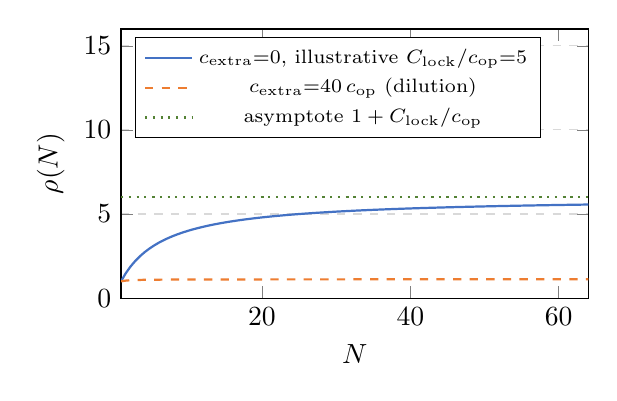
\begin{tikzpicture}
\begin{axis}[
    width=0.62\textwidth, height=5cm,
    xlabel={$N$}, ylabel={$\rho(N)$},
    xmin=1, xmax=64,
    ymin=0, ymax=16,
    ymajorgrids, grid style={dashed, gray!30},
    legend pos=north west, legend style={font=\scriptsize},
    domain=1:64, samples=100,
]
\addplot[curveA, thick] {x*(5+1)/(5+x)};
\addlegendentry{$c_{\mathrm{extra}}{=}0$, illustrative $C_{\mathrm{lock}}/c_{\mathrm{op}}{=}5$}
\addplot[curveB, thick, dashed] {x*(5+1+40)/(5+x*41)};
\addlegendentry{$c_{\mathrm{extra}}{=}40\,c_{\mathrm{op}}$ (dilution)}
\addplot[curveC, dotted, thick] {1 + 5/(1)} ;
\addlegendentry{asymptote $1+C_{\mathrm{lock}}/c_{\mathrm{op}}$}
\end{axis}
\end{tikzpicture}
\caption{Qualitative shape of $\rho(N)$ under Claim~\ref{claim:rho},
with illustrative (not fitted) parameter values chosen only to display
the predicted shape: monotonic increase toward a finite asymptote when
$c_{\mathrm{extra}}{=}0$ (solid), collapsing toward $\rho{\approx}1$
once a large workload-identical per-entry cost $c_{\mathrm{extra}}$ is
introduced (dashed). No curve here is fit to
\S\ref{sec:eval:perf}'s measured values; the comparison against those
values is made qualitatively, point-by-point, in the itemized list
above.}
\label{fig:rho-model}
\end{figure}

\subsection{Orthogonality of the Two Axes}
\label{sec:theory:orthogonal}

The runtime model of \S\ref{sec:theory:runtime} concerns $C_{\mathrm{lock}}$
and $c_{\mathrm{op}}$ under a \emph{fixed} locking protocol; it says
nothing about \emph{contention} between concurrent cursors, which is
the separate, well-understood mechanism behind
\S\ref{sec:eval:gap1}'s finding that \corten{coarse} degrades to
35--50\% of \corten{rw}'s throughput under multiple threads (a single
global lock serializes what fine-grained locking allows to proceed in
parallel --- an instance of Amdahl's-law-style critical-section
contention, not of the amortization argument in
\S\ref{sec:theory:principle}). The proof-obligation model
(\S\ref{sec:theory:proof}) and the interface-removal runtime model
(\S\ref{sec:theory:runtime}) both concern a \emph{single} cursor's
lock-acquisition discipline and are silent on contention. This
separation is exactly what makes the $2{\times}2$ matrix
(Table~\ref{tab:matrix}) a valid factorial design rather than a
confound: locking granularity (degenerate/structural, governing
contention \emph{and}, via Claim~\ref{claim:threshold}, the proof
threshold) and interface style (transactional/non-transactional,
governing $\rho(N)$ via Claim~\ref{claim:rho}) are modeled, and
observed, as independent axes.

\subsection{Scope and Non-Claims}
\label{sec:theory:scope}

We are explicit about what \S\ref{sec:theory:proof}--\ref{sec:theory:orthogonal}
do \emph{not} claim to explain, so as not to overreach beyond
\S\ref{sec:eval}'s evidence:

\begin{itemize}
  \item \textbf{No claim about intermediate lock granularities.} We
    built and measured exactly two points on the degenerate/structural
    axis (Observation~\ref{obs:degenerate}); Figure~\ref{fig:threshold}
    depicts a binary distinction, not a continuum we have data for. A
    protocol locking, say, every other level is not covered by
    Claim~\ref{claim:threshold} as stated.
  \item \textbf{No claim about the residual tooling issues.} The two
    residual failures reported in
    \S\ref{sec:eval:threats} are, by our own diagnosis there, properties
    of Verus's SMT-facing trigger/fact-propagation machinery, not of
    the logical proof obligation our model concerns; neither model in
    this section makes any prediction about either, and none should be
    inferred.
  \item \textbf{No claim of numerical calibration.} Every reference to
    the runtime model's parameters ($C_{\mathrm{lock}}$,
    $c_{\mathrm{op}}$, $c_{\mathrm{extra}}$) in this section is
    qualitative; we did not estimate their values from
    \S\ref{sec:eval:perf}'s data via regression, and
    Figure~\ref{fig:rho-model}'s curves use illustrative parameters
    chosen for legibility, not fitted ones.
  \item \textbf{No claim beyond CortenMM's own two protocols.} The
    threshold effect (\S\ref{sec:theory:proof}) is stated for and
    checked against \corten{rw}/\corten{rcu}, the only two structural
    protocols in our artifact; \S\ref{sec:eval:threats}'s independent-system
    finding (that no external candidate we examined exposes the
    transactional/non-transactional axis at all) means the model has
    not been checked, in either direction, outside CortenMM itself.
\end{itemize}



\section{Related Work}
\label{sec:related}

We organize related work around the same four-axis classification of
the memory-management design space that motivated this project's
initial literature analysis of CortenMM, so that each system we
discuss --- and each of the seven variants evaluated in
\S\ref{sec:eval} --- can be located precisely relative to it.

\subsection{The Design Space: A Four-Axis Classification}
\label{sec:related:mece}

We classify a page-table/memory-management design along four
mutually exclusive, collectively exhaustive axes:

\begin{itemize}
  \item \textbf{A --- Abstraction layering:} \emph{2-level} (a
    higher-level VMA/mapping structure and a separate, independently
    reasoned-about hardware page table, as in Linux and most
    textbook designs) vs.\ \emph{1-level} (a single structure that
    \emph{is} the hardware page table, as CortenMM proposes, collapsing
    the two).
  \item \textbf{B --- Concurrency protocol:} \emph{coarse} (one lock for
    the whole structure), \emph{fine-rw} (per-node/per-level
    reader--writer locking), \emph{RCU} (read-copy-update with
    epoch-based reclamation), or \emph{replication} (per-core replicas
    synchronized through an operation log, as in node replication).
  \item \textbf{C --- Interface atomicity:} \emph{non-transactional}
    (each operation independently acquires and releases whatever
    locks it needs, as in Linux) vs.\ \emph{transactional} (a single
    handle is acquired once and shared across a caller-chosen sequence
    of operations, as CortenMM's cursor design and
    \S\ref{sec:method:cursor} describe).
  \item \textbf{D --- Correctness methodology:} \emph{testing} (the
    traditional approach), \emph{core-verified} (the core
    data-structure and locking-protocol invariants are
    machine-checked, as CortenMM and this paper's variants are, in
    Verus), or \emph{whole-system-verified} (functional correctness of
    the entire kernel is machine-checked end-to-end, as in seL4).
\end{itemize}

This gives $2 \times 4 \times 2 \times 3 = 48$ cells; a system or
artifact occupies exactly one. Figure~\ref{fig:mece-grid} positions
CortenMM's own published variant, the Verus-verified relatives we are
aware of, and every variant we built in \S\ref{sec:method:variants},
within the $B \times C$ slice at $A{=}1\text{-level}$,
$D{=}\text{core-verified}$ --- the slice this paper's experiments live
in.

\begin{figure}[h]
\centering
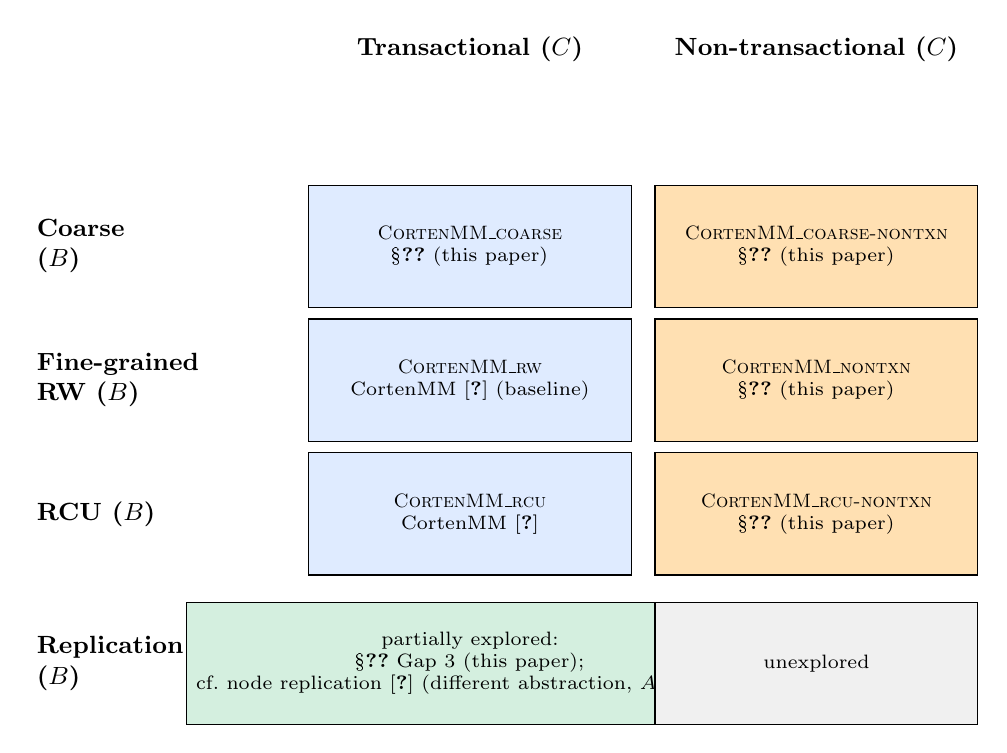
\begin{tikzpicture}[
    hdr/.style={font=\bfseries\small, align=center},
    cell/.style={draw, minimum width=4.1cm, minimum height=1.55cm, align=center, font=\scriptsize},
]
\node[hdr] at (4.4,0.9) {Transactional ($C$)};
\node[hdr] at (8.8,0.9) {Non-transactional ($C$)};

\node[hdr, align=left, text width=2.2cm] at (0,-1.6) {Coarse\\($B$)};
\node[cell, fill=priorcol] (c11) at (4.4,-1.6)
  {\corten{coarse}\\\S\ref{sec:eval:gap1} (this paper)};
\node[cell, fill=thispapercol] (c12) at (8.8,-1.6)
  {\corten{coarse-nontxn}\\\S\ref{sec:eval:gap4} (this paper)};

\node[hdr, align=left, text width=2.2cm] at (0,-3.3) {Fine-grained\\RW ($B$)};
\node[cell, fill=priorcol] (c21) at (4.4,-3.3)
  {\corten{rw}\\CortenMM~\cite{cortenmm} (baseline)};
\node[cell, fill=thispapercol] (c22) at (8.8,-3.3)
  {\corten{nontxn}\\\S\ref{sec:eval:gap4} (this paper)};

\node[hdr, align=left, text width=2.2cm] at (0,-5.0) {RCU ($B$)};
\node[cell, fill=priorcol] (c31) at (4.4,-5.0)
  {\corten{rcu}\\CortenMM~\cite{cortenmm}};
\node[cell, fill=thispapercol] (c32) at (8.8,-5.0)
  {\corten{rcu-nontxn}\\\S\ref{sec:eval:rcu} (this paper)};

\node[hdr, align=left, text width=2.2cm] at (0,-6.9) {Replication\\($B$)};
\node[cell, fill=partialcol] (c41) at (4.4,-6.9)
  {partially explored:\\\S\ref{sec:eval} Gap~3 (this paper);\\cf.\ node
  replication~\cite{nr} (different abstraction, $A{=}2$-level)};
\node[cell, fill=opencol] (c42) at (8.8,-6.9)
  {unexplored};
\end{tikzpicture}
\caption{The $B \times C$ slice at $A{=}1\text{-level}$,
$D{=}\text{core-verified}$. Blue cells were built and published by the
CortenMM paper itself~\cite{cortenmm}; orange cells are this paper's
own ablations (\S\ref{sec:method:variants}); the green cell is partially
explored (this paper's Gap~3, which combines replication with a
transactional interface but was not carried to the same completeness
as the other cells); the gray cell is, to our knowledge, unexplored in
the $1$-level/core-verified region entirely. The entire
non-transactional column (right) is this paper's contribution: every
cell in it was empty before \S\ref{sec:eval}.}
\label{fig:mece-grid}
\end{figure}

\subsection{Verified Memory Management and the Abstraction Axis ($A$)}
\label{sec:related:abstraction}

CortenMM's central claim~\cite{cortenmm} is that collapsing $A$ from
2-level to 1-level is what makes core-level verification of a
performant page table tractable at all; \S\ref{sec:eval:gap1}
corroborates this from the opposite direction, holding $A{=}1$-level
fixed and showing that verification cost is essentially insensitive to
$B$ (\corten{coarse} vs.\ \corten{rw}, 142 vs.\ 149 obligations) ---
i.e., $A$, not $B$, is where CortenMM's verifiability advantage lives,
exactly as the original paper argues, now with the $B$-axis held
constant as a control.

Prior verified kernels sit at different points on $A$ and $D$
simultaneously, which is why none directly overlaps with our
experiments. \textsc{seL4}~\cite{sel4} is whole-system-verified
($D{=}$whole-system) but its memory management is capability-based
with a comparatively simple, largely static mapping structure, not a
dynamically-locked, concurrently-mutated page table in CortenMM's or
Linux's sense; its proof effort is dominated by axes this paper does
not vary. \textsc{CertiKOS}~\cite{certikos} verifies a layered kernel
where each abstraction layer is itself a separate refinement target
--- a form of $A$ taken to an extreme (many levels, each verified
independently) rather than CortenMM's collapse to one. Neither system
provides the controlled, same-codebase comparison this paper's
ablations require; both differ from our baseline on $A$, $D$, and
often $B$ simultaneously, so a proof-cost comparison against them would
confound exactly the variables \S\ref{sec:method:principle}'s
methodology is designed to isolate.

The $A$ axis itself predates verification as a concern: Talluri,
Hill, and Khalidi's clustered page
table~\cite{clustered-pagetable} is an early instance of collapsing
structure to reduce overhead --- associating several pages' mapping
information with one radix-tree entry to reduce memory footprint ---
motivated entirely by hardware/cache efficiency, decades before
CortenMM's collapse of the same axis was motivated by proof
tractability. That the same axis recurs as a lever for two
historically distinct goals (memory efficiency then, verifiability
now) is, we think, suggestive that $A$ is a genuinely fundamental
design axis rather than one CortenMM introduces; we do not, however,
ablate it ourselves (\S\ref{sec:eval:gap1} holds it fixed throughout),
so this connection is offered as context, not as part of this paper's
evidence.

\subsection{Concurrency Protocols and Their Verification ($B$)}
\label{sec:related:concurrency}

\S\ref{sec:eval:rcu} is, to our knowledge, the first controlled
comparison of proof cost for the \emph{same} interface-atomicity
ablation ($C$) across two different points on the $B$ axis within one
verified artifact. Prior verification work on individual concurrency
protocols exists for each point on $B$ in isolation: RCU's semantics
have been given formal treatments outside the page-table setting (most
directly relevant to CortenMM\_rcu's own reclamation-set reasoning,
\S\ref{sec:eval:rcu}, is the general line of work formalizing
grace-period and epoch-based reclamation soundness); reader--writer
lock protocols are among the most extensively verified concurrency
primitives in the Verus ecosystem, of which CortenMM\_rw is one
instance; and node replication --- $B{=}$replication --- has its own
verified treatment in \textsc{verified-node-replication}~\cite{nr},
built atop a verified implementation of the underlying \textsc{NrOS}
technique~\cite{nros}, and a verified kernel building on the same
replication idea, \textsc{verified-nrkernel}~\cite{nrkernel}. Both of
the latter sit at $A{=}2$-level (a replicated log-structured design
distinct from CortenMM's single-layer collapse) and, as
\S\ref{sec:eval:threats} reports, neither exposes the $C$-axis
distinction this paper ablates: \vfn{verified-nrkernel} is
single-threaded (no $B$-protocol contention to speak of, hence no
transactional-interface question), and node replication's public
interface (\vfn{execute}/\vfn{execute\_mut}) is per-operation by
construction, occupying only the non-transactional column of
Figure~\ref{fig:mece-grid} by design, with no transactional counterpart
to ablate against. This is precisely the observation
\S\ref{sec:eval:threats} reports as a threat to
generalization --- not that our finding is contradicted by these
systems, but that they do not instantiate the axis needed to test it.

CortenMM's own performance evaluation compares against two further,
unverified points on $B$ that sit outside our classification's
core-verified column ($D{=}$testing) but are worth situating precisely.
\textsc{RadixVM}~\cite{radixvm} takes yet another approach to
concurrent address-space management: rather than locking a shared
tree at any granularity, it replicates the page table per core and
uses a radix-tree metadata structure with distributed reference
counting to let non-overlapping \vfn{mmap}/\vfn{munmap} operations
proceed with zero cache-coherence traffic --- a design point
CortenMM's own evaluation reports as achieving excellent scalability
at the cost of the per-core replication's memory overhead. RadixVM's
\vfn{mmap}/\vfn{munmap} interface is, like Linux's, non-transactional;
whether \S\ref{sec:theory:proof}'s threshold effect applies to it is a
question our classification cannot answer without first asking whether
per-core replication's own locking discipline has the single-write,
bounded-ancestor-range structure \S\ref{sec:method:cursor} identifies
as the effect's precondition --- RadixVM's radix tree, unlike
CortenMM's, is not shared across cores at all, which may place it
outside the threshold effect's scope entirely rather than on one side
or the other of it. We leave this open rather than speculate further,
since RadixVM has no proof to ablate around in the first place.

\subsection{Interface Atomicity in Systems Verification ($C$)}
\label{sec:related:atomicity}

The transactional/non-transactional distinction we ablate is a
verification-specific instance of a much older systems question:
whether an interface should expose a session-like handle amortized
across operations, or re-establish preconditions on every call.
Database and transactional-memory systems have studied the
\emph{performance} side of this trade-off extensively; our contribution
is specific to its \emph{proof-cost} side, and specifically to the
mechanism identified in \S\ref{sec:theory:proof}: that transactional
handles let an implementation leave a frame-preservation obligation
\emph{implicit}, and that removing them is precisely what forces it to
become explicit, enumerable, and single-write-site-local
(\S\ref{sec:method:sites}). We are not aware of prior work that
isolates interface atomicity as an independent axis of verification
cost, separate from the concurrency protocol or abstraction layer it
sits atop --- which is what motivates $C$ as its own axis in
Figure~\ref{fig:mece-grid}, rather than folding it into $B$.

\subsection{Ablation and Differential Methodology in Verification
Research}
\label{sec:related:methodology}

Verification-preserving ablation (\S\ref{sec:method:principle}) is
methodologically closest to \emph{differential} or \emph{controlled
comparison} studies in systems research --- work that holds most of a
system fixed and varies one design decision to attribute an effect ---
but applies the idea specifically to \emph{proof engineering effort} as
the measured quantity, rather than runtime performance alone. Two
distinct existing traditions bear on this choice of measured quantity,
and both differ from our approach in the same way: neither performs a
controlled, same-codebase ablation against a variant differing in
exactly one axis. The first tradition reports a single system's
\emph{total} verification cost, typically in person-time: seL4's own
published accounting (roughly 12 person-years for the functional
correctness proof, about 25 for the full initial
project)~\cite{sel4-proof-eng}, and IronFleet's reported 3.7
person-years for two complete distributed
systems~\cite{ironfleet}, are figures about \emph{one} artifact's
absolute cost, not a decomposition of which of that artifact's design
decisions contributed how much of it. The second tradition studies
proof \emph{productivity} as a general phenomenon --- Staples et
al.~\cite{proof-productivity} mine effort and proof-size records across
nine projects in the L4.verified family and find a strong linear
relationship between the two, informing cost \emph{estimation} for
future projects of similar shape --- but again without attributing
cost to individual, independently variable design axes within one
system, which is the specific gap this paper's methodology addresses.
Winter's survey of the field~\cite{qed-at-large} catalogs the broader
practice of \emph{proof engineering} that both traditions belong to; we
position verification-preserving ablation as a technique within that
practice, specialized to the attribution question rather than to
absolute cost measurement or productivity estimation.

A retrofit of a non-transactional interface onto Linux --- a system at a
different point on $D$ entirely (testing, not core-verified) --- served
a complementary role in the broader project this paper is drawn from:
not as a proof-cost ablation (Linux has no proof to measure the cost
of), but as an independent, executable check that the
frame-preservation concern \S\ref{sec:method:repair} identifies as
CortenMM's motivation for transactional locking corresponds to a real
hazard (a genuine deadlock reproduced in a Linux kernel module) outside
the verified setting altogether.

\subsection{The Rust Deductive Verification Ecosystem}
\label{sec:related:rust-ecosystem}

Verus~\cite{verus}, the tool CortenMM and every variant in this paper
is verified with, is one of several deductive verifiers that have
emerged for Rust in recent years, each making a different choice about
where to sit on the automation/expressiveness trade-off surveyed by Le
Blanc et al.~\cite{rust-verification-survey}. Prusti~\cite{prusti}
verifies safe Rust by translating into the Viper intermediate
verification language and specifying mutable borrows via
\emph{pledges}; Creusot~\cite{creusot} takes a similar
safe-Rust-focused approach via translation into Why3's WhyML,
specifying mutable borrows via \emph{prophecy variables} instead ---
the two tools' main point of divergence, per Le Blanc et
al.~\cite{rust-verification-survey}. Both differ from Verus's approach
(linear ghost types integrated directly into the Rust type system,
checked against an SMT backend) in requiring translation to a
separate intermediate verification language; whether this affects the
proof-engineering patterns \S\ref{sec:method:sites} identifies ---
the step-fact/transitivity pattern is stated in terms of Verus's own
\vfn{forall}/\vfn{assert} constructs and \vfn{=\textasciitilde{}=}
extensional-equality operator specifically --- is a question this
paper does not address; we are not aware of a page-table-scale
verified artifact in Prusti or Creusot against which the same ablation
could currently be attempted. Kani~\cite{kani} occupies a different
point entirely, using bounded model checking rather than deductive
verification, trading unbounded functional-correctness guarantees for
substantially lower annotation burden; CortenMM's own core proof
obligations --- and the frame-preservation property this paper's
ablations turn on --- are unbounded loop-invariant properties of the
kind bounded model checking does not, in general, establish, which is
why CortenMM chose, and this paper stays within, the deductive family.


\section{Conclusion}
\label{sec:conclusion}

We set out to answer a question CortenMM's own publication does not:
given a verified system that bundles a single-layer abstraction,
fine-grained locking, and a transactional interface, which decision
buys which of its reported properties? Verification-preserving
ablation --- copy the baseline byte-for-byte, change exactly one axis,
verify with the identical toolchain --- let us answer it with the same
precision Verus itself demands of the proofs we ablated around.

The answer is not ``the transactional interface has a fixed proof
cost.'' It is a threshold effect: the cost exists, and is substantial
(9~sites, $\sim$150 lines, \S\ref{sec:eval:gap4}), precisely when the
underlying locking protocol requires reasoning about an ancestor range
that can genuinely vary at runtime, and it vanishes --- not shrinks,
\emph{vanishes}, to the same obligation count, \S\ref{sec:eval:gap4}'s
$142$ vs.\ $142$ --- when that range is degenerate. The same
threshold reappears, independently derived and independently repaired,
in an entirely separate concurrency protocol (\S\ref{sec:eval:rcu}),
which is the strongest evidence we can offer within one artifact that
we identified a property of \emph{tree-traversal-based fine-grained
concurrency control} and not an accident of CortenMM\_rw's specific
code. The runtime side of the same story (\S\ref{sec:eval:perf},
\S\ref{sec:theory:runtime}) is real, sizeable, and equally conditional:
large when lock acquisition dominates the work being done, and diluted
toward parity once it does not.

Neither finding required a new system, a new proof, or a new
benchmark harness invented from scratch --- only the discipline of
holding everything but one design axis fixed, and the patience to
enumerate, by hand, every place a proof obligation that used to be
implicit had to be written down. We think that discipline generalizes
beyond CortenMM: any verified system whose interface amortizes a
protocol-acquisition cost across a caller-chosen operation sequence is
a candidate for the same ablation, and our threshold-effect and
amortized-cost models (\S\ref{sec:theory}) make falsifiable,
checkable predictions about what such an ablation should find. What we
could not do is check those predictions against a second, independent
system: of the externally verified Verus artifacts we examined
(\S\ref{sec:eval:threats}, \S\ref{sec:related:concurrency}), none
exposes the transactional/non-transactional axis at all. Whether that
absence reflects a genuine rarity of the design choice, or simply the
small number of systems we could check, is a question this paper
raises but leaves open. We see three concrete directions building on
this work: applying verification-preserving ablation to a system built
independently of CortenMM, once one instantiating the interface-atomicity
axis is available; resolving the two residual tooling
limitations that keep three of our six variants from a clean
0-error result, which \S\ref{sec:eval:threats} diagnoses precisely
enough to be independently reproducible; and extending the runtime
model of \S\ref{sec:theory:runtime} to multi-core contention, which the
present work deliberately keeps separate from the interface-removal
question it isolates.


\begin{thebibliography}{99}

\bibitem{cortenmm}
Junyang Zhang, Xiangcan Xu, Yonghao Zou, Zhe Tang, Xinyi Wan, Kang Hu,
Siyuan Wang, Wenbo Xu, Di Wang, Hao Chen, Lin Huang, Shoumeng Yan,
Yuval Tamir, Yingwei Luo, Xiaolin Wang, Huashan Yu, Zhenlin Wang,
Hongliang Tian, and Diyu Zhou.
\newblock CortenMM: Efficient Memory Management with Strong
Correctness Guarantees.
\newblock In \emph{Proceedings of the ACM SIGOPS 31st Symposium on
Operating Systems Principles (SOSP~'25)}, pages 1082--1098, Seoul,
Republic of Korea, October 2025. ACM. Best Paper Award.

\bibitem{sel4}
Gerwin Klein, Kevin Elphinstone, Gernot Heiser, June Andronick,
David Cock, Philip Derrin, Dhammika Elkaduwe, Kai Engelhardt,
Rafal Kolanski, Michael Norrish, Thomas Sewell, Harvey Tuch, and
Simon Winwood.
\newblock seL4: Formal Verification of an OS Kernel.
\newblock In \emph{Proceedings of the ACM SIGOPS 22nd Symposium on
Operating Systems Principles (SOSP~'09)}, pages 207--220, Big Sky,
MT, USA, October 2009. ACM.

\bibitem{certikos}
Ronghui Gu, Zhong Shao, Hao Chen, Xiongnan (Newman) Wu, Jieung Kim,
Vilhelm Sj\"oberg, and David Costanzo.
\newblock CertiKOS: An Extensible Architecture for Building Certified
Concurrent OS Kernels.
\newblock In \emph{Proceedings of the 12th USENIX Symposium on
Operating Systems Design and Implementation (OSDI~'16)}, pages
653--669, Savannah, GA, USA, November 2016. USENIX Association.

\bibitem{nros}
Ankit Bhardwaj, Chinmay Kulkarni, Reto Achermann, Irina Calciu,
Sanidhya Kashyap, Ryan Stutsman, Amy Tai, and Gerd Zellweger.
\newblock NrOS: Effective Replication and Sharing in an Operating
System.
\newblock In \emph{Proceedings of the 15th USENIX Symposium on
Operating Systems Design and Implementation (OSDI~'21)}, pages
295--312, July 2021. USENIX Association.

\bibitem{nrkernel}
Matthias Brun et al.
\newblock \texttt{verified-nrkernel}: a Verus-verified, single-threaded
page-table implementation modeled on NrOS's page-table management.
\newblock Software artifact.
\newblock \url{https://github.com/matthias-brun/verified-nrkernel}.

\bibitem{nr}
The Verus Project Contributors.
\newblock \texttt{verified-node-replication}: a Verus-verified
implementation of the node-replication (NR) concurrent-data-structure
replication technique.
\newblock Software artifact.
\newblock \url{https://github.com/verus-lang/verified-node-replication}.

\bibitem{verus}
Andrea Lattuada, Travis Hance, Chanhee Cho, Matthias Brun,
Isitha Subasinghe, Yi Zhou, Jon Howell, Bryan Parno, and
Chris Hawblitzel.
\newblock Verus: Verifying Rust Programs using Linear Ghost Types.
\newblock In \emph{Proceedings of the 34th Annual ACM Conference on
Object-Oriented Programming, Systems, Languages, and Applications
(OOPSLA~'23)}, Lisbon, Portugal, October 2023. ACM.

\bibitem{sel4-proof-eng}
Gerwin Klein.
\newblock Proof Engineering Considered Essential.
\newblock In \emph{Proceedings of the 19th IFIP World Congress
(WCC~2014)}, volume 8442 of \emph{LNCS}, pages 16--21. Springer, 2014.

\bibitem{proof-productivity}
Mark Staples, Rafal Kolanski, Gerwin Klein, Corey Lewis,
June Andronick, Toby Murray, Ross Jeffery, and Len Bass.
\newblock Productivity for Proof Engineering.
\newblock In \emph{Proceedings of the 8th ACM/IEEE International
Symposium on Empirical Software Engineering and Measurement
(ESEM~'13)}, Baltimore, MD, USA, October 2013. ACM.

\bibitem{qed-at-large}
Talia Ringer.
\newblock \emph{QED at Large: A Survey of Engineering of Formally
Verified Software}.
\newblock arXiv:2003.06458, 2020.

\bibitem{ironfleet}
Chris Hawblitzel, Jon Howell, Manos Kapritsos, Jacob R.\ Lorch,
Bryan Parno, Michael L.\ Roberts, Srinath Setty, and Brian Zill.
\newblock IronFleet: Proving Practical Distributed Systems Correct.
\newblock In \emph{Proceedings of the 25th ACM Symposium on Operating
Systems Principles (SOSP~'15)}, pages 1--17, Monterey, CA, USA,
October 2015. ACM.

\bibitem{rust-verification-survey}
Alex Le Blanc, Patrick Lam, and Nurit Karassik.
\newblock Surveying the Rust Verification Landscape.
\newblock arXiv:2410.01981, 2024.

\bibitem{prusti}
Peter M\"uller, Federico Poli, and Alexander J.\ Summers.
\newblock The Prusti Project: Formal Verification for Rust.
\newblock In \emph{NASA Formal Methods Symposium (NFM~2022)}, volume
13260 of \emph{LNCS}, pages 88--108. Springer, 2022.

\bibitem{creusot}
Xavier Denis, Jacques-Henri Jourdan, and Claude March\'e.
\newblock The Creusot Environment for the Deductive Verification of
Rust Programs.
\newblock Technical report, Inria, 2021.

\bibitem{kani}
The Kani Rust Verifier Contributors.
\newblock Kani: A Bounded Model Checker for Rust.
\newblock Software artifact and documentation.
\newblock \url{https://github.com/model-checking/kani}.

\bibitem{radixvm}
Austin T.\ Clements, M.\ Frans Kaashoek, and Nickolai Zeldovich.
\newblock RadixVM: Scalable Address Spaces for Multithreaded
Applications.
\newblock In \emph{Proceedings of the 8th ACM European Conference on
Computer Systems (EuroSys~'13)}, pages 211--224, Prague, Czech
Republic, April 2013. ACM.

\bibitem{clustered-pagetable}
Madhusudhan Talluri, Mark D.\ Hill, and Yousef A.\ Khalidi.
\newblock A New Page Table for 64-Bit Address Spaces.
\newblock In \emph{Proceedings of the 15th ACM Symposium on Operating
Systems Principles (SOSP~'95)}, pages 184--200, Copper Mountain, CO,
USA, December 1995. ACM.

\end{thebibliography}

\appendix
\section{Artifact}
\label{sec:artifact}

We describe the structure and honest scope of the artifact
accompanying this paper (repository: \vfn{artifact-repo/}), organized
to let a reviewer independently re-verify every number reported in
\S\ref{sec:eval}.

\subsection{Contents}

\begin{itemize}
  \item \textbf{\vfn{benchmarks/}} --- the complete, exact source of
    all three performance-benchmark C programs
    (\vfn{mmap\_batch\_scale.c}, \vfn{mprotect\_scale.c},
    \vfn{alloc\_arena\_scale.c}) underlying every runtime number in
    \S\ref{sec:eval:perf}, together with the raw, per-run \texttt{rdtsc}
    cycle-count data as CSV files (including every repeated run
    discussed there for the \vfn{mmap} $N{\in}\{16,64\}$ and
    \vfn{mprotect} $N{=}64$ points) and a CSV summary of every
    variant's verification-obligation/error count
    (Tables~\ref{tab:gap1-proof}, \ref{tab:gap4-proof},
    \ref{tab:matrix}, \ref{tab:rcu-proof}).
  \item \textbf{\vfn{patches/}} --- the exact, complete diffs applied
    to go from each transactional baseline to its non-transactional
    counterpart: the \vfn{wf\_push\_level} fix
    (\S\ref{sec:method:repair}), the complete \vfn{nontxn\_api.rs}
    wrapper file (\S\ref{sec:method:sites}), the RCU-specific
    \vfn{sub\_tree\_rt}/\vfn{is\_root} patches
    (\S\ref{sec:eval:rcu}), and the full site-by-site inventory of
    every place the step-fact/transitivity pattern was applied
    (Table~\ref{tab:variants-sites}).
  \item \textbf{\vfn{docs/}} --- environment setup notes; the four
    independent artifact-infrastructure findings referenced in the
    paper's Introduction (contributions list), each with root cause
    and workaround/fix; and a full writeup of the residual
    \vfn{InstanceId}-equality Verus tooling limitation
    (\S\ref{sec:eval:threats}), including the exact failing diagnostic
    and the two remedies attempted against it
    (\texttt{\#[verifier::rlimit(n)]} and
    \texttt{\#[verifier::spinoff\_prover]}).
  \item \textbf{\vfn{scripts/}} --- the exact commands used to
    (re-)verify all six variants and to (re-)run all three benchmarks.
\end{itemize}

\subsection{What this artifact does not contain, and why}

This artifact does \emph{not} include the complete source of the six
verified Verus crates themselves --- each is several thousand lines,
only a fraction of which this paper's ablations touch. \corten{rw}
and \corten{rcu} are CortenMM's own published baselines and should be
obtained from the CortenMM artifact directly; the four ablated
variants are reconstructed by applying \vfn{patches/} to copies of the
appropriate baseline, exactly as \vfn{scripts/verify\_all\_variants.sh}
describes. We chose to ship precise, complete, independently-checkable
\emph{patches} against a well-defined base, rather than a full
snapshot of six large crates transcribed from working notes,
specifically to avoid the risk of a transcription error in files large
enough that such an error could go unnoticed; every patch in this
artifact was independently checked for internal consistency (e.g.\ that
every reported overhead ratio in the benchmark CSVs recomputes exactly
from its own batched/per-page cycle counts) before being included here.

\subsection{Reproducing the central claims}

\begin{itemize}
  \item \textbf{Table~\ref{tab:matrix} (the $2{\times}2$ matrix).}
    Building all four crates and reading each \texttt{cargo xtask
    verify} summary line reproduces $149/142/150/142$.
    Corollary~\ref{cor:coarse-nontxn} (zero new proof code for the
    degenerate-protocol cell) is checkable directly: \corten{coarse-nontxn}
    is constructed by transplanting \corten{nontxn}'s \vfn{mod.rs}
    verbatim onto \corten{coarse}'s \vfn{locking.rs}, with no
    additional edit.
  \item \textbf{The RCU correspondence (Table~\ref{tab:rcu-correspondence}).}
    The specific missing \vfn{forall} range in \corten{rcu}'s original
    \vfn{wf\_push\_level}, and the single-clause fix that repairs it,
    are recorded as a standalone patch
    (\vfn{patches/rcu-to-rcu-nontxn/}), independent from, but
    line-for-line matching, the same fix applied to \corten{rw}
    (\vfn{patches/rw-to-nontxn/}), so that ``the same fix'' is a claim
    about two inspectable diffs, not a prose characterization.
\end{itemize}

\subsection{Known limitations of the artifact}

Consistent with \S\ref{sec:eval:threats}, this artifact does not claim
0 verification errors for \corten{nontxn}, \corten{coarse-nontxn}, or
\corten{rcu-nontxn}; it documents exactly the 2-, 3-, and 3-error
residual states \S\ref{sec:eval} reports for these three variants
respectively, each involving two distinct tooling-limitation classes
(\S\ref{sec:eval:tooling}), with the specific failing clauses
identified in \vfn{docs/verus-tooling-issue.md} and, for
\corten{coarse-nontxn}, a complete raw diagnostic transcript in
\vfn{docs/verification\_log\_coarse\_nontxn.txt}. That documentation
also records a finer distinction not stated elsewhere in the paper:
\corten{nontxn}'s \vfn{query\_locked} reaches a clean 0-error result,
while neither \corten{coarse-nontxn}'s nor \corten{rcu-nontxn}'s does
(all three of each variant's wrapper functions hit at least one of the
two residual issues). \emph{Post-submission reproduction note:} both
the proof-cost reproduction path
(\vfn{scripts/verify\_all\_variants.sh}) and the runtime-benchmark
path (\vfn{scripts/run\_benchmarks.sh}) have since been independently
confirmed to reproduce end-to-end. The proof-cost path reproduces exit
code 0 and all six variants' exact obligation/error counts as reported
above. The runtime-benchmark path initially encountered an
intermittent kernel-image build failure, root-caused to a
registry-mirror-shadowing conflict for
\vfn{osdk-frame-allocator}/\vfn{osdk-heap-allocator}/\vfn{ostd}
(full diagnosis in \vfn{docs/environment-setup-and-findings.md}, issue
4) rather than the originally-suspected \vfn{cargo-osdk}
build-provenance issue; a permanent fix (patching these three crates
to their local workspace paths) is now applied automatically by
\vfn{scripts/run\_benchmarks.sh}, after which all three benchmark
programs reproduced overhead ratios consistent with
\vfn{benchmarks/raw\_data\_*.csv} within the paper's documented
run-to-run noise band. This artifact does not include a build of an
external, independently maintained Verus artifact instantiating both
sides of the interface-atomicity axis, since --- per
\S\ref{sec:eval:threats} --- we did not find one; a reviewer wishing to
extend \S\ref{sec:theory}'s threshold-effect prediction to such a
system would need to construct the ablation themselves, using
\S\ref{sec:method} as a template.


\end{document}
